\documentclass[TheoreticalPhy_ModB.tex]{subfiles}
\begin{document}


\chapter{QED Processes at Lowest order} %Sei stato bravissimo, si chiamava proprio così

\section{The QED Lagrangian and its Symmetries}
\textsf{Mandl, sec 11.1 - Maggiore, sec 7.1}\\
Quantum electrodynamic (QED) describes the interactions between (or any other charged spin 1/2 particle) and photons. QED is described by the lagrangian
\[
\mathL_{\text{QED}} =\underbrace{\overline{\psi }( i\slashed \partial -m) \psi }_{\mathcal{L}^{( 0)}_{D}} \ -\underbrace{\frac{1}{4} F_{\mu \nu } F^{\mu \nu }}_{\mathcal{L}_{EM}} -\underbrace{qA_{n}\overline{\psi } \gamma ^{\mu } \psi }_{\mathcal{L}_{int}} -\underbrace{\frac{1}{2\xi }\left( \partial _{\mu } A^{\mu }\right)^{2}}_{\mathcal{L}_{GF}}
%Vengono un po' una merda le graffe sotto quindi vedi tu se vuoi tenerele o fare in un altro modo
\]
\begin{enumerate}
\item $\mathL_D^{(0)}$ is the langrangian for the free Dirac field
\item $\mathL_{EM}$ is the lagrangian for the free EM field. In order to quatize the E-n field we have to add the term $\mathL_{GF}$ (gauge fixing). For other purposes this term can be omitted. Usually the choice $\xi = 1$, called Feynman gauge, is the simplest choice for quantization
\item $\mathL_{int}$ describes the interaction between Dirac field and EM-field. Notice that the term $\mathL_D = \mathL_D^{(0)} + \mathL_{int}$ can be obtained from $\mathL_D^{(0)}$ with the ``minimal substitution'' $\partial_{\mu} \to \partial_{\mu} + iqA_{\mu} = D_{\mu}$, i.e. using covariant derivative $D_{\mu}$ instead of $\partial_{\mu}$ in the dirac lagrangian.\\
Notice that $\mathL_D$ exhibits local symmetry, while $\mathL_D^{(0)}$ doesn't
\end{enumerate}
Besides Lorentz invariance, the QED exhibits following symmetries:
\begin{enumerate}[label=$\bullet$]
\item \textbf{Global U(1) symmetry}
\[
\begin{cases}
\psi(x) \to \psi'(x) = e^{i \alpha}\psi(x) \qquad \alpha \in \mathR \\
A^{\mu}(x) \to A^{\prime \mu}(x) = A^{\mu}(x)
\end{cases}
\]
There is therefore an associated conserved Noether current
\[
j^{\mu} = q \overline{\psi} \gamma^{\mu} \psi
\quad \to \quad
\partial_{\mu}j^{\mu} = 0 
\]
and a U(1) charge which is conserved by the EM interaction
\[
Q = q \int \de^3 x \ \psi^{\dagger} \psi
\qquad
\frac{\de Q}{\de t} = 0
\]
\item \textbf{Local U(1) symmetry} (gauge symmetry)
\[
\begin{cases}
\psi(x) \to \psi'(x) = e^{iq\alpha(x)} \psi(x) \\
A^{\mu} \to A^{\prime \mu}(x) = A^{\mu}(x) - iq\partial^{\mu}\alpha(x)
\end{cases}
\]
notice that the global U(1) symmetry is a sequence of the local U(1) symmetry, taking $\alpha(x)$ constant)\\ \\
The covariant derivative of $\psi$ $D_{\mu}\psi$ behaves as a spinor (remember that $D_{\mu}$ transforms as a vector):
\[
\begin{split}
D_{\mu}\psi \to (D_{\mu}\psi)' = D'_{\mu}\psi'	& = (D_{\mu} - iq\partial_{\mu} \alpha)(e^{iq\alpha(x)} \psi(x)) \\
	& = (\partial_{\mu} + iqA_{\mu} - iq\partial_{\mu}\alpha)(e^{iq\alpha} \psi) \\
	& = e^{iq\alpha}(\partial_{\mu} + iqA_{\mu})\psi \\
	& = e^{iq\alpha(x)}(D_{\mu}\psi)
\end{split}
\]
This implies that $\mathL_D$ is invariant. Since $\mathL_{EM}$ is invariant, the full lagrangian is invariant
\end{enumerate}

\section{Flavors in QED and the SU(3) Flavor Global Symmetry}
QED describes interactions of the photon field with several kind of leptons, not only electron and positrons. Particles that differs only by their mass are called \textbf{flavours}.
\skipline
The next table describes leptons in QED. There are two families of leptons that differs by their charge. We indicate with (-) (minus) particles with negative charge, and with (+) (plus) particles with positive charge (antiparticles)\\
\skipline
Flavours in QED
\[
\begin{array}{l | cccccc}
\toprule
Leptons \footnotemark	& e 		& \mu 	& \tau 	& \nu_e 		& \nu_{\mu} 	& \nu_{\tau} \\
\midrule
q					& -1		& -1		& -1		& 0			& 0			& 0 \\
m [MeV]				& 0.5		& 105	& 1777	& \simeq 0		& \simeq 0		& \simeq 0 \\
\bottomrule
\end{array}
\]
\footnotetext{Neutrinos admit anly global U(l) symmetry \\
Neutrino masses are in the order $m_{\nu} \approx 10^{-6} me \le 1 eV$}
\skipline
The dirac lagrangian $\mathL_D$ can be modified in order to consider all possible leptons
\[
\mathL_D = \sum_{i=1}^n \bar{\psi_i} (i \slashed D - m_i) \psi_i
	\simeq \sum_{i=1}^{n_l} \bar{\psi_i} (i \slashed D - m_i) \psi_i
	+ \sum_{j=1}^{n_n} \bar{\psi_i} (i \slashed \partial) \psi_i
\]
with $n$: number of leptons, $n_l$: number of electrically charged particles, $n_n$: number of neutrinos.\\
In the last term the interaction term vanishes because of q=0\\
If we adopt a matrix notation
\begin{align}
\Psi_C & =
\begin{pmatrix}
\psi_e \\
\psi_{\mu} \\
\psi_{\tau}
\end{pmatrix}
&
\Psi_N & =
\begin{pmatrix}
\psi_{\nu_e} \\
\psi_{\nu_{\mu}} \\
\psi_{\nu_{\tau}}
\end{pmatrix}
\notag \\
\bar{\Psi}_C & = (\bar{\psi_e}, \bar{\psi_{\mu}}, \bar{\psi_{\tau}})
&
\bar{\Psi}_N & = (\bar{\psi}_{\nu_e}, \bar{\psi}_{\nu_{\mu}}, \bar{\psi}_{\nu_{\tau}})
\notag 
\end{align}
The subscript C stands for ``charged'', and N for ``neutral''\\
We can define following matrices
\[
M_C =
\begin{pmatrix}
m_e 	& 0 			& 0 \\
0	& m_{\mu}	& 0 \\
0	& 0			& m_{\tau}
\end{pmatrix}
\qquad
Q_C = (-1) \id_{3 \times 3}
\qquad
M_N \simeq Q_N = \emptyset_{3 \times 3}
\]
and the generalization of the covariant derivative $D_{\mu} = \partial_{\mu} \cdot \id_{3 \times 3} + iA_{\mu}Q_C$ we obtain
\[
\mathL_D = \underbrace{\bar{\Psi}_C (i \slashed D - M_C)\Psi_C}_{\mathL_C} +
	\underbrace{\bar{\Psi}_N(i \slashed \partial \id_{3 \times 3})\Psi_N}_{\mathL_N}
\]
The term $\mathL_C$ and $\mathL_N$ are respectively the \textbf{Charged Sector} and the \textbf{Neutral Sector} of $\mathL_D$\\
The basis defined by $\Psi_C$ and $\Psi_N$ is called \textbf{physical basis}, since physical particles are identified by their mass.

\subsection{Global Symmetry of Neutral and Charged Sector}
Let's consider a U(3) transformation
\[
\Psi(x) \to \Psi'(x) = U\Psi(x)
\qquad
U^{\dagger}U = \id_{3 \times 3}
\]
Spinors and vector are left invariant\\
The neutral sector is left invariant under U(3) tfm
\[
\mathL_N \to \mathL'_N = \bar{\Psi'}_N (i \slashed \partial \id_{3 \times 3})\Psi'_N =
	\bar{\Psi}_N U^{\dagger}(i \slashed \partial \id_{3 \times 3})U \Psi_N = \mathL_N
\]
The charged sector is not invariant because of the mass term
\[
\mathL \to \mathL'_C = \bar{\Psi}_C ( i \slashed D - U^{\dagger}M_C U)\Psi_C \ne \mathL_C
\quad \textup{in general}
\]
In order to obtain global symmetries of the flavor QED lagrangian, we search the subgroup of U(3) made by matrices $U-g$ that satisfies
\begin{equation}
U^{\dagger}_g M_C U_g = M_c
\qquad
U_g \in U(3)
\label{eq:U3}
\end{equation}
We can prove that $U(3) \overset{isomorphism}{\simeq} U(1) \times SU(3)$, with
\begin{enumerate}
\item |det(U(3)| = 1
\item det(U(1)) = $e^{i\theta}$ \footnote{Indicando con $e^{i\theta}$ il determinante delle matrici $U_g \in U(3)$}
\item det(SU(3)) = 1 \footnote{SU(3) è l'insieme di livello dato da $(\arg \circ \textup{ det})^{-1}(0)$}
\end{enumerate}
Since generators of SU(3) are Gell-Mann matrices $\lambda_a$ (for a = $1, \dots, 8$), generators of U(3) are
\[
\id \times \{ \lambda_1, \dots, \lambda_8 \}
\]
we can also prove that equation \ref{eq:U3} is satisfied only by diagonal matrix\\
Diagonal generators of SU(3) are
\[
\lambda_0 =
\begin{pmatrix}
1	& 0 	& 0 \\
0	& 1	& 0 \\
0	& 0	& 1
\end{pmatrix}
\qquad
\lambda_3 =
\begin{pmatrix}
1	& 0 	& 0 \\
0	& -1	& 0 \\
0	& 0	& 0
\end{pmatrix}
\qquad
\lambda_8 =
\begin{pmatrix}
1	& 0 	& 0 \\
0	& 1	& 0 \\
0	& 0	& -2
\end{pmatrix}
\]
Up to a phase, matrices $U_g$ are in the form
\[
U_g = e^{i \alpha_0 \lambda_0} \ e^{i \alpha_3 \lambda_3} \ e^{i \alpha_8 \lambda_8}
\]
For i = 0, 3 ,8 we have $[\lambda_i, M_c] = 0$ and then the equation \ref{eq:U3} is satisfied: if we take $\alpha_i \ll 1$
\[
(1 - i \alpha_i \lambda_i)M_C(1 + i \alpha_i \lambda_i) = (M_C - i \alpha_i [\lambda_i, M_C] + o(\alpha_i^2)) \simeq M_C
\]
We then obtained that the global group of symmetry is generated by the algebra
\[
\mathcal{G} = \{ \lambda_0, \lambda_3, \lambda_8 \} = U(1)^3 \subset U(3)
\]
I define the following basic of $\mathcal{G}$:
\[
\lambda_e =
\begin{pmatrix}
1	& 0 	& 0 \\
0	& 0	& 0 \\
0	& 0	& 0
\end{pmatrix}
\qquad
\lambda_{\mu} =
\begin{pmatrix}
0	& 0 	& 0 \\
0	& 1	& 0 \\
0	& 0	& 0
\end{pmatrix}
\qquad
\lambda_{\tau} =
\begin{pmatrix}
0	& 0 	& 0 \\
0	& 0	& 0 \\
0	& 0	& 1
\end{pmatrix}
\]
These matrices generates phase tfm for each kind of leptons ($\lambda_e$ generates phase tfm for e, ecc $\dots$)\\
Conserved quantities of this group are 3, and corresponding to the number of particles of each type (Antiparticles are counted with negative sign)\\
\begin{example}
$\mu^- \to e^- \gamma$ is forbidden in QED. 
This is an example of conserved charges due to unitary symmetry that have nothing to do with electric charge.\\
Flavours changing in neutral sector are forbidden too
\end{example}

\section{QED Feynman Rules $\to$ fogli stampati (23-26)}

\section{$e^+ e^- \to f^+ f^-$}
This diagram is called s-channel
\begin{equation*}
\begin{tikzpicture}[layered layout, baseline=(nu)]
  \begin{feynman}[large]
    \vertex (f1) {\(e^-\)};
    \vertex [label={[label distance=0.12cm]180:$\mu$}] at ([shift={(315:2.5)}]f1) (mu);
    \vertex [below left=of mu] (b1) {\(e^+\)};
    \vertex [label={[label distance=0.12cm]2:$\nu$}] at ([shift={(0:3.2)}]mu) (nu);
    \vertex [above right=of nu] (f2) {\(f^-\)};
    \vertex [below right=of nu] (b2) {\(f^+\)};

    \diagram*{
      (f1) -- [fermion, momentum={[arrow shorten=0.2]\(p\)}] (mu)
      		-- [photon, edge label'={\(k=p'+q'\)}, momentum={[arrow shorten=0.3]\(k=p+q=\sqrt{s}\)}] (nu)
      		-- [fermion, momentum={[arrow shorten=0.2]\(p'\)}] (f2),
      (b1) -- [anti fermion, momentum'={[arrow shorten=0.25]\(q\)}] (mu),
      (nu) -- [fermion, momentum'={[arrow shorten=0.25]\(q'\)}] (b2),
    };
  \end{feynman}
\end{tikzpicture}
\end{equation*}
With $k=p' + q'$ we impose the 4 momentum conservation\\
We have
\[
S_{fi} = (2 \pi)^4 \delta^4 (p+q-p'-q')\mathM_{fi}
\]
with Feynman amplitude
\[
\begin{split}
\mathM_{fi}	& = (-iq)^2 \bigl[ \bar{u}_{r'}(p') \gamma^{\nu} \ v_{s'}(q') \bigr] \footnotemark
					\bigl[ \bar{v}_s(q) \gamma^{\mu} \ u_r(p) \bigr] \footnotemark
					D^{F}_{\mu \nu}(k) \\
			& = (-iq)^2 \frac{-ig_{\mu \nu}}{k^2 + i \epsilon} \ \bigl[ \bar{u}_{r'} (p') \gamma^{\nu} \ v_{s'}(q') \bigr]
					\bigl[ \bar{v}_s (q) \gamma^{\mu} \ u_r(p) \bigr] \\
			& = \frac{iq^2}{s + i\epsilon} \ \bigl[ \bar{u}_{r'}(p') \gamma_{\mu} \ v_{s'}(q') \bigr]
					\bigl[ \bar{v}_s(q) \gamma^{\mu} \ u_r(p) \bigr]
\end{split}
\]
\footnotetext{indica il percorso $e^- \to \mu \to e^+$ nel diagramma}
\footnotetext{indica il percorso $f^- \to \nu \to f^+$ nel diagramma}
In the second passage $\xi =1$. We can prove that this choice has no importance, \textsf{see Maggiore pg 187}\\ \\
Using the identity $(\bar{u} \gamma^{\mu} v)^* = \bar{v} \gamma^{\mu} u$ (that can be proved by direct calculation using
$(\gamma^{\mu})^{\dagger} = \gamma^0 \gamma^{\mu} \gamma^0$) we obtain (we omit polarization indexes)
\todo{gurda foglio 27}
\[
\begin{split}
\abs{\mathM_{fi}}^2 = \mathM_{fi} \mathM^*_{fi}	& = \frac{q^4}{s^2} \bigl( \bar{u}(p')\gamma_{\mu} v(q') \bigr) \
											\bigl( \bar{v}(q) \gamma^{\mu}u(p) \bigr) \\
										& = ??
\end{split}
\]
At this point, we are still free to specify any particular spinors $u_r(p)$, $\bar{v}_{s'}(p')$ and so on, corresponding to any desired spin states of the fermions.

\subsection{Sum Over Fermion Spins. Squared Averaged Feynman Amplitude}
The Feynman amplitude simplifies considerably when we throw away the spin information. We want to compute
\[
\abs{\overline{\mathM_{fi}}}^2 = \underbrace{\frac{1}{2} \sum_s \ \frac{1}{2} \sum_r}_{\textup{average over} \atop \text{the initial states}} \ 
	\underbrace{\sum_{s'} \ \sum_{r'}}_{\textup{sum over} \atop \text{final states}} \abs{\mathM(r,s \to r',s')}^2
\]
This sum can be performed using completeness relations for dirac spinors
\[
\sum_r u_s(p) \bar{u}_s(p) = \slashed p + m
\qquad
\sum_s v_s(p) \bar{v}_s(p) = \slashed p - m
\]
Writing spinors indexes explicitly 
\[
\begin{split}
\sum_{rs} \text{e-current}	& = \sum_{rs} \bar{v}^s_a(q) (\gamma^{\mu})_{ab} \, u^r_b(p) \, \bar{u}^r_c(p) (\gamma^{\nu})_{cd} \, v_d^s(q) \\
					& = (\slashed q - m)_{da} \, \gamma^{\mu}_{ab} \, (\slashed p + m)_{bc} \, \gamma_{cd}^{\nu} \\
					& = \Tr \bigl[ (\slashed q - m) \gamma^{\mu} (\slashed p + m) \gamma^{\nu} \bigr]
\end{split}
\]
and similarly
\[
\sum_{r's'} \text{f-current} = \Tr \bigl[ (\slashed p' + m) \gamma_{\mu} (\slashed q' - m)\gamma_{\nu} \bigr]
\]
So we obtain
\[
\overline{\abs{\mathM_{fi}}^2} = \frac{q^4}{4s^2} \Tr \bigl[ (\slashed q - m) \gamma^{\mu} (\slashed p + m) \gamma^{\nu} \bigr]
	\Tr \bigl[ (\slashed p' + m) \gamma_{\mu} (\slashed q' -m) \gamma_{\nu} \bigr]
\]
The spinors u and v have disappeared, leaving us with a much cleaner expression in terms of $\gamma$ matrices. This trick is very genera: any QED amplitude involving external fermions, when squared and summed or averaged over spins, can be converted in this way to traces of products of Dirac matrices

\skipline
There is a trick to obtain previous formula using only Feynman rules. If we set $\mathM_{fi}=\mathM_e\mathM_f$ (we divide $\mathM_{fi}$ in 2 factors related to e and f), then $\abs{\mathM_{fi}}^2 = \mathM_e^* \mathM_e \, \mathM_f^* \mathM_f$. We have
\todo{Da completare}
\begin{equation*}\sum_{rs} \mathM^*_e \, \mathM_e=%
\begin{tikzpicture}[baseline=(nu)]
  \begin{feynman}[large]
    \vertex [label={[label distance=0.1cm]2:$\nu$}] at ([shift={(315:2.5)}]f1) (nu);
    \vertex [left=of nu] (f1) {};
    \vertex [label={[label distance=0.12cm]180:$\mu$}] at ([shift={(0:3.2)}]nu) (mu);
    \vertex [right=of mu] (f2) {};

    \diagram*{
      (f1) -- [photon, momentum'={[arrow shorten=0.2]\(k\)}] (nu),
      (nu) -- [fermion, half left, momentum'={[arrow shorten=0.25]\(p\)}] (mu),
      (mu) -- [fermion, half left, momentum'={[arrow shorten=0.25]\(q\)}] (nu),
      (mu) -- [photon, momentum'={[arrow shorten=0.25]\(k\)}] (f2),
    };
  \end{feynman}
\end{tikzpicture}
\end{equation*}
The closed fermion line contributes in the final amplitude with a factor
\[
\frac{q^2}{2s} \Tr \bigl[ \underbrace{(\slashed p + m)}_{\textup{Fermion}} \gamma^{\nu} \underbrace{(\slashed q - m)}_{\textup{Antifermion}} \gamma^{\mu} \bigr]
\]
The factor $-q^2/(2s)$ is obtained using full diagram (s is given by photon propagator)
\todo{Fare diagramma di Feynman}

\skipline
Going back to the expression of $\abs{\mathM_{fi}}^2$ that we obtain, now we need to calculate explicitly $\gamma$ matrices traces
\[
\Tr \bigl[ (\slashed p + m) \gamma^{\nu} (\slashed q - m) \gamma^{\mu} \bigr] =
\Tr \bigl[ \slashed p \ \gamma^{\nu} \slashed q \ \gamma^{\mu} \bigr] - m^2 \Tr [\gamma^{\nu} \ \gamma^{\mu} ] +
m \bigl( \Tr [\gamma^{\nu} \slashed q \ \gamma^{\mu} ] - \Tr [ \slashed p \ \gamma^{\nu} \gamma^{\mu}] \bigr)
\]
Now we prove some properties of $\gamma-$matrices traces (\textsf{other properties in Peskin pg 133-135})
\begin{enumerate}[label=(\Roman*)]
\item 
	\begin{alignat*}{2}
	\Tr [\gamma^{\mu}] 	& = \Tr[\gamma^5 \, \gamma^5 \, \gamma^{\mu} ]		&\quad & \to (\gamma^5)^2 = \id \\
						& = - \Tr [ \gamma^5 \, \gamma^{\mu} \, \gamma^5 ]	&& \to \{ \gamma^5, \gamma^{\mu} \} = 0 \\
						& = - \Tr [ \gamma^5 \, \gamma^5 \, \gamma^{\mu} ] 	&& \to \textup{cyclicity} \\
						& = -\Tr[\gamma^{\mu}] 							&& \\
						& \so \Tr [\gamma^{\mu}] = 0						&&						
	\end{alignat*}
\item
	\begin{align*}
	\Tr [\gamma^{\mu} \, \gamma^{\nu} \, \gamma^{\rho} \, \gamma^{\sigma}]
	&= \Tr [2g^{\mu\nu} \, \gamma^{\rho}\, \gamma^{\sigma} - \gamma^{\nu}\, \gamma^{\mu}\, \gamma^{\rho}\, \gamma^{\sigma} ] \\
	& = 2g^{\mu\nu} \Tr[ \gamma^{\rho}\, \gamma^{\sigma}] - \Tr[\gamma^{\nu}2g^{\mu\rho}\gamma^{\sigma}
		- \gamma^{\nu}\, \gamma^{\rho}\, \gamma^{\mu}\, \gamma^{\sigma}] \\
	& = 8g^{\mu\nu}g^{\rho\sigma} - 8g^{\mu\rho}g^{\nu\sigma} +
		\Tr[\gamma^{\nu}\, \gamma^{\rho}\, 2g^{\mu\sigma} - \gamma^{\nu}\, \gamma^{\rho}\, \gamma^{\sigma}\, \gamma^{\mu}] \\
	& = 8 \bigl( g^{\mu\nu}g^{\rho\sigma} - g^{\mu\rho}g^{\nu\sigma} + g^{\mu\sigma}g^{\nu\rho} \bigr)
		-\Tr[\gamma^{\mu}\, \gamma^{\nu}\, \gamma^{\rho}\, \gamma^{\sigma}] \\
	& \so \Tr[\gamma^{\mu}\, \gamma^{\nu}\, \gamma^{\rho}\, \gamma^{\sigma}] =
		4\bigl( g^{\mu\nu}g^{\rho\sigma} - g^{\mu\rho}g^{\nu\sigma} + g^{\mu\sigma}g^{\nu\rho} \bigr)
	\end{align*}
\end{enumerate}

From previous calculation, using induction, can be easily proved that $\Tr[\underbrace{\gamma^{\mu} \dots \gamma^{\sigma}}_{\textup{odd \# of} \atop \gamma \textup{ matrices}}] = 0$\\
With these relations we obtain
\begin{enumerate}[label=$\bullet$]
\item
	\begin{align*}
	\Tr[(\slashed p + m) \gamma^{\nu}(\slashed q - m) \gamma^{\sigma}]
	& = 4(g^{\mu\nu}g^{\rho\sigma} - g^{\mu\rho}g^{\nu\sigma} + g^{\mu\sigma}g^{\nu\rho}) p_{\mu}q_{\rho} - m^2 4g^{\nu\sigma} \\
	& = 4 (p^{\nu}q^{\sigma} - g^{\nu\sigma}p \cdot q + p^{\sigma}q^{\nu} - g^{\nu\sigma}m^2) \\
	& = 4 \bigl(p^{\nu}q^{\sigma} + p^{\sigma}q^{\nu} - g^{\nu\sigma}(p \cdot q + m^2) \bigr) \\
	& \textup{with m = mass of }e^I
	\end{align*}
\item
	\[
	\Tr [(\slashed p' + m) \gamma_{\mu} (\slashed q' - m) \gamma_{\nu}]
		= 4 \bigl( p'_{\mu} \, q'_{\nu} + p'_{\nu}\, q'_{\mu} \, g_{\mu\nu}(p' \cdot q' + M^2) \bigr)
	\qquad \text{with M = mass of } f^I
	\]
\item
	\begin{align*}
	\overline{\abs{\mathM_{fi}}^2} 
	& = \frac{4q^4}{s^2} \, \bigl( p^{\mu}q^{\nu} + p^{\nu}q^{\mu} - g^{\mu\nu}(p \cdot q + m^2) \bigr)
		\bigl( p'_{\mu}\, q'_{\nu} + p'_{\nu}\, q_{\mu} - g_{\mu\nu} (p' \cdot q' + M^2) \bigr) \\
	& \approx \frac{8q^4}{s^2} \bigl( (p \cdot p')(q \cdot q') + (p \cdot q')(p' \cdot q) + M^2(p \cdot q) \bigr)
		\qquad \textup{if } m \ll M
	\end{align*}
\end{enumerate}
To obtain a more explicit formula we must specialize to a particular frame of reference and express the vectors $p, q, p', q', k$ in terms of the basis kinematic variables (energies and angles) in that frame. In practice, the choice of frame will be dictated by the experimental conditions.\\
We want to calculate cross section in the center of mass frame.

\todo{Cambia il nome del file}
\todo{Da sistemare}
\begin{figure}[H]
\centering


\tikzset{every picture/.style={line width=0.75pt}} %set default line width to 0.75pt        

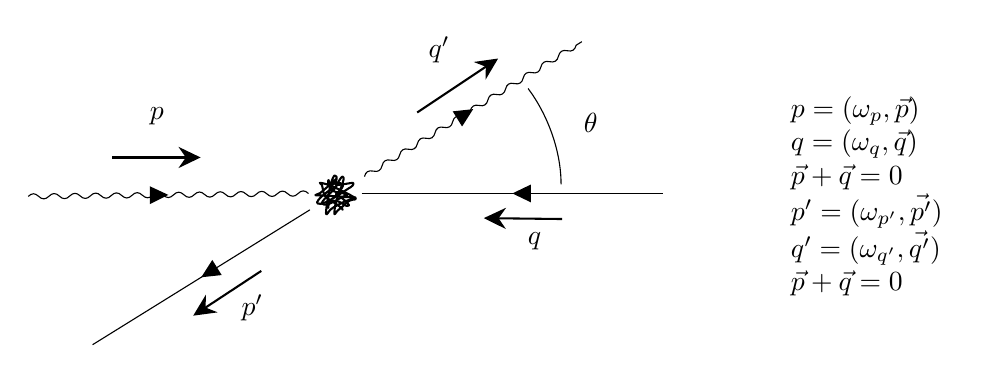
\begin{tikzpicture}[x=0.75pt,y=0.75pt,yscale=-1,xscale=1]
%uncomment if require: \path (0,300); %set diagram left start at 0, and has height of 300

%Straight Lines [id:da2201162405089543] 
\draw    (94,144.56) .. controls (95.65,142.87) and (97.31,142.85) .. (99,144.5) .. controls (100.68,146.15) and (102.35,146.13) .. (104,144.45) .. controls (105.65,142.77) and (107.32,142.75) .. (109,144.4) .. controls (110.69,146.05) and (112.35,146.03) .. (114,144.34) .. controls (115.65,142.66) and (117.32,142.64) .. (119,144.29) .. controls (120.69,145.94) and (122.35,145.92) .. (124,144.23) .. controls (125.65,142.55) and (127.32,142.53) .. (129,144.18) .. controls (130.68,145.83) and (132.35,145.81) .. (134,144.13) .. controls (135.65,142.44) and (137.31,142.42) .. (139,144.07) .. controls (140.68,145.72) and (142.35,145.7) .. (144,144.02) .. controls (145.65,142.34) and (147.32,142.32) .. (149,143.97) .. controls (150.69,145.62) and (152.35,145.6) .. (154,143.91) .. controls (155.65,142.23) and (157.32,142.21) .. (159,143.86) .. controls (160.68,145.51) and (162.35,145.49) .. (164,143.81) .. controls (165.65,142.12) and (167.31,142.1) .. (169,143.75) .. controls (170.68,145.4) and (172.35,145.38) .. (174,143.7) .. controls (175.65,142.02) and (177.32,142) .. (179,143.65) .. controls (180.69,145.3) and (182.35,145.28) .. (183.99,143.59) .. controls (185.64,141.91) and (187.31,141.89) .. (188.99,143.54) .. controls (190.67,145.19) and (192.34,145.17) .. (193.99,143.49) .. controls (195.64,141.8) and (197.3,141.78) .. (198.99,143.43) .. controls (200.67,145.08) and (202.34,145.06) .. (203.99,143.38) .. controls (205.64,141.7) and (207.31,141.68) .. (208.99,143.33) .. controls (210.68,144.98) and (212.34,144.96) .. (213.99,143.27) .. controls (215.64,141.59) and (217.31,141.57) .. (218.99,143.22) .. controls (220.67,144.87) and (222.34,144.85) .. (223.99,143.17) .. controls (225.64,141.48) and (227.3,141.46) .. (228.99,143.11) -- (229.06,143.11) -- (229.06,143.11) ;
\draw [shift={(161.53,143.83)}, rotate = 539.39] [fill={rgb, 255:red, 0; green, 0; blue, 0 }  ][line width=0.08]  [draw opacity=0] (8.93,-4.29) -- (0,0) -- (8.93,4.29) -- cycle    ;
%Straight Lines [id:da8440776864610582] 
\draw    (256,135) .. controls (256.54,132.71) and (257.96,131.83) .. (260.25,132.36) .. controls (262.54,132.9) and (263.96,132.02) .. (264.5,129.73) .. controls (265.03,127.44) and (266.45,126.56) .. (268.74,127.09) .. controls (271.03,127.62) and (272.45,126.74) .. (272.99,124.45) .. controls (273.53,122.16) and (274.95,121.28) .. (277.24,121.82) .. controls (279.53,122.35) and (280.95,121.47) .. (281.49,119.18) .. controls (282.03,116.89) and (283.45,116.01) .. (285.74,116.54) .. controls (288.03,117.08) and (289.45,116.2) .. (289.99,113.91) .. controls (290.52,111.62) and (291.94,110.74) .. (294.23,111.27) .. controls (296.52,111.8) and (297.94,110.92) .. (298.48,108.63) .. controls (299.02,106.34) and (300.44,105.46) .. (302.73,106) .. controls (305.02,106.53) and (306.44,105.65) .. (306.98,103.36) .. controls (307.52,101.07) and (308.94,100.19) .. (311.23,100.72) .. controls (313.52,101.25) and (314.94,100.37) .. (315.47,98.08) .. controls (316.01,95.79) and (317.43,94.91) .. (319.72,95.45) .. controls (322.01,95.98) and (323.43,95.1) .. (323.97,92.81) .. controls (324.51,90.52) and (325.93,89.64) .. (328.22,90.17) .. controls (330.51,90.71) and (331.93,89.83) .. (332.47,87.54) .. controls (333.01,85.25) and (334.43,84.37) .. (336.72,84.9) .. controls (339.01,85.43) and (340.43,84.55) .. (340.96,82.26) .. controls (341.5,79.97) and (342.92,79.09) .. (345.21,79.63) .. controls (347.5,80.16) and (348.92,79.28) .. (349.46,76.99) .. controls (350,74.7) and (351.42,73.82) .. (353.71,74.35) .. controls (356,74.89) and (357.42,74.01) .. (357.96,71.72) -- (360.72,70) -- (360.72,70) ;
\draw [shift={(308.36,102.5)}, rotate = 508.17] [fill={rgb, 255:red, 0; green, 0; blue, 0 }  ][line width=0.08]  [draw opacity=0] (8.93,-4.29) -- (0,0) -- (8.93,4.29) -- cycle    ;
%Straight Lines [id:da09307133911969756] 
\draw    (254.67,143.11) -- (399.83,143.11) ;
\draw [shift={(327.25,143.11)}, rotate = 0] [fill={rgb, 255:red, 0; green, 0; blue, 0 }  ][line width=0.08]  [draw opacity=0] (8.93,-4.29) -- (0,0) -- (8.93,4.29) -- cycle    ;
%Curve Lines [id:da33812291607616296] 
\draw    (334.83,92.56) .. controls (343.5,104.11) and (350.72,121.44) .. (350.72,138.78) ;
%Straight Lines [id:da5774490131113152] 
\draw [line width=0.75]    (134.44,125.78) -- (174.06,125.78) ;
\draw [shift={(177.06,125.78)}, rotate = 180] [fill={rgb, 255:red, 0; green, 0; blue, 0 }  ][line width=0.08]  [draw opacity=0] (10.72,-5.15) -- (0,0) -- (10.72,5.15) -- (7.12,0) -- cycle    ;
%Straight Lines [id:da24269378260147034] 
\draw [line width=0.75]    (281.39,104.11) -- (317.89,79.78) ;
\draw [shift={(320.39,78.11)}, rotate = 506.31] [fill={rgb, 255:red, 0; green, 0; blue, 0 }  ][line width=0.08]  [draw opacity=0] (10.72,-5.15) -- (0,0) -- (10.72,5.15) -- (7.12,0) -- cycle    ;
%Straight Lines [id:da3757335905736008] 
\draw [line width=0.75]    (206.28,180.44) -- (176.01,200.35) ;
\draw [shift={(173.5,202)}, rotate = 326.66999999999996] [fill={rgb, 255:red, 0; green, 0; blue, 0 }  ][line width=0.08]  [draw opacity=0] (10.72,-5.15) -- (0,0) -- (10.72,5.15) -- (7.12,0) -- cycle    ;
%Straight Lines [id:da04091628549293125] 
\draw    (125,216) -- (229.72,151) ;
\draw [shift={(177.36,183.5)}, rotate = 328.17] [fill={rgb, 255:red, 0; green, 0; blue, 0 }  ][line width=0.08]  [draw opacity=0] (8.93,-4.29) -- (0,0) -- (8.93,4.29) -- cycle    ;
%Straight Lines [id:da587248071756918] 
\draw [line width=0.75]    (351.28,155.44) -- (316.5,155.04) ;
\draw [shift={(313.5,155)}, rotate = 360.66999999999996] [fill={rgb, 255:red, 0; green, 0; blue, 0 }  ][line width=0.08]  [draw opacity=0] (10.72,-5.15) -- (0,0) -- (10.72,5.15) -- (7.12,0) -- cycle    ;
%Shape: Free Drawing [id:dp672077562881797] 
\draw  [color={rgb, 255:red, 0; green, 0; blue, 0 }  ][line width=0.75] [line join = round][line cap = round] (238.5,139) .. controls (238.5,134.42) and (238.79,137.16) .. (239.5,140) .. controls (239.61,140.46) and (240.17,139.33) .. (240.5,139) .. controls (241.52,137.98) and (244.74,137.49) .. (245.5,139) .. controls (246.37,140.74) and (240.56,144) .. (242.5,144) .. controls (244.25,144) and (249.12,148.69) .. (248.5,149) .. controls (246.85,149.82) and (245.13,147.33) .. (243.5,147) .. controls (242.19,146.74) and (240.69,146.4) .. (239.5,147) .. controls (238.56,147.47) and (238.5,151.05) .. (238.5,150) .. controls (238.5,145.09) and (238.54,139.96) .. (241.5,137) .. controls (241.83,136.67) and (242.5,136) .. (242.5,136) .. controls (242.5,136) and (235.39,142.55) .. (234.5,143) .. controls (233.83,143.33) and (231.75,144) .. (232.5,144) .. controls (238.77,144) and (245.98,145) .. (251.5,145) .. controls (253.3,145) and (248.11,146.2) .. (246.5,147) .. controls (244.9,147.8) and (240.81,149.69) .. (239.5,151) .. controls (238.83,151.67) and (237.73,153.91) .. (237.5,153) .. controls (237.11,151.43) and (240.32,130.65) .. (242.5,135) .. controls (243.1,136.19) and (241.39,138.26) .. (242.5,139) .. controls (243.03,139.35) and (250.31,137.81) .. (250.5,138) .. controls (251.19,138.69) and (249.76,139.87) .. (249.5,140) .. controls (247.14,141.18) and (236.38,149.44) .. (233.5,148) .. controls (231.39,146.95) and (240.55,140) .. (242.5,140) ;
%Shape: Free Drawing [id:dp3629185907562005] 
\draw  [color={rgb, 255:red, 0; green, 0; blue, 0 }  ][line width=0.75] [line join = round][line cap = round] (245.5,151) .. controls (245.5,149.77) and (238.43,145.93) .. (237.5,145) .. controls (235.85,143.35) and (236.16,140.97) .. (235.5,139) .. controls (235.35,138.55) and (234.03,138) .. (234.5,138) .. controls (237.62,138) and (245.48,141.99) .. (247.5,143) .. controls (248.99,143.75) and (253.17,146) .. (251.5,146) .. controls (247.23,146) and (245.77,149.87) .. (243.5,151) .. controls (242.66,151.42) and (241.5,153.94) .. (241.5,153) .. controls (241.5,147.47) and (243.79,143.12) .. (245.5,138) .. controls (245.82,137.05) and (246.39,135.45) .. (245.5,135) .. controls (244.77,134.63) and (241.54,140.96) .. (241.5,141) .. controls (240.88,141.62) and (234.76,147.26) .. (235.5,148) .. controls (237.89,150.39) and (245.38,144) .. (247.5,144) .. controls (248.25,144) and (246.21,143.24) .. (245.5,143) .. controls (243.55,142.35) and (241.34,142.84) .. (239.5,141) ;

% Text Node
\draw (365,109) node    {$\theta $};
% Text Node
\draw (156,106) node    {$p$};
% Text Node
\draw (292,74) node    {$q'$};
% Text Node
\draw (202,198) node    {$p'$};
% Text Node
\draw (338,166) node    {$q$};
% Text Node
\draw (498,145) node    {$ \begin{array}{l}
p = (\omega_p, \vec{p}) \\
q = (\omega_q, \vec{q}) \\
\vec{p} + \vec{q} = 0 \\
p' = (\omega_{p'}, \vec{p'})\\
q' = (\omega_{q'}, \vec{q'}) \\
\vec{p} + \vec{q} = 0
\end{array}$};


\end{tikzpicture}
\end{figure}

In the CM frame we have following kinematics relations
\[
\left.
\begin{aligned}
(p + q)	& = (\omega_p + \omega_q, \vec{p} + \vec{q}) = (\omega_p + \omega_q, 0) \\
s 		& = (p + q)^2 = (\omega_p + \omega_q)^2
\end{aligned}
\right \} = (p + q) = (\sqrt{s}, 0)
\]
and
\[
\omega_p = (p + q)^2 = (\omega_p + \omega_q)^2
\]
Same for final momenta
\begin{gather*}
(p' + q') = (\sqrt{s}, 0) \\
\omega_{p'} = \omega_{q'} = \frac{\sqrt{s}}{2}
\end{gather*}
For product momenta
\begin{align*}
(p \cdot q) 		& = \omega^2 - \vec{p}\vec{q} = \omega^2 \abs{\vec{p}}^2 = 2 \omega^2 - m^2 
	\overset{m=0}{\simeq} 2\omega^2 \\
(p' \cdot q') 		& = \omega^2 - \vec{p}\vec{q} = \omega^2 \abs{\vec{p}}^2 = 2 \omega^2 - M^2 \notag \\
(p \cdot p') 		& = \omega^2 - \vec{p}\vec{p'} = \omega^2 - \abs{\vec{p}}\abs{\vec{p'}}\cos \theta 
	\overset{m = 0}{\simeq} \omega(\omega - \abs{\vec{p'}} \cos \theta)
	\overset{m = 0}{\simeq} (q \cdot q') \\
(p \cdot q')		& = \omega^2 + \vec{p}\, \vec{p'} = \omega^2 + \abs{\vec{p}}\abs{\vec{p'}}\cos \theta 
	\simeq \omega(\omega + \abs{\vec{p'}}\cos \theta) \simeq (q \cdot p') \\
\abs{\vec{p'}}^2 	& = \omega^2 - M^2 = \omega^2 \biggl( 1 - \frac{M^2}{\omega^2} \biggr)
	= \frac{s}{4} \biggl( 1 - \frac{4M^2}{s} \biggr) \\
\abs{\vec{p}}^2 	& = \omega^2 + m^2 \overset{m = 0}{\simeq} \omega^2 = \frac{s}{4}
\end{align*}
Now we can rewrite $\overline{\abs{\mathM_{fi}}^2}$ in terms of $\omega$ and $\theta$. If $m=0$ is valid (e.g. $m_e/m_{\mu} = 1/200$)
\begin{align*}
\overline{\abs{\mathM_{fi}}^2}
	& \simeq \frac{8q^4}{s^2} \bigl[ (\omega^4 - 2 \omega^3 \abs{p'} \cos \theta + \omega^2 \abs{p'}^2 \cos^2 \theta) 
		+ (\omega^4 + 2 \omega^3 \abs{p'} \cos \theta + \omega^2 \abs{p'}^2 \cos^2 \theta) + 2M^2\omega^2 \bigr] \\
	& = \frac{8q^4}{s^2} \biggl[ \frac{2s}{4} \biggl( \frac{s}{4} + \frac{s}{4} \biggl( 1 - \frac{4M^2}{s} \biggr) \cos^2 \theta \biggr)
		+ 2M^2 \frac{s}{4} \biggr]	\\
	& = q^4 \biggl[ \biggl( 1 + \frac{4M^2}{s} \biggr) + \biggl( 1 - \frac{4M^2}{s} \biggr) \cos^2 \theta \biggr] 				 
\end{align*}
Cross section formula in the CM frame reads
\begin{align}
\biggl( \frac{\de \bar{\sigma}}{\de \Omega} \biggr)_{CM}
	& = \frac{1}{64\pi^4} \ \frac{1}{s} \ \frac{\abs{p'}}{\abs{q'}} \ \abs{\overline{\mathM}}^2_{CM} \notag \\
	& = \frac{q^4}{64 \pi^2} \ \frac{1}{s} \ \biggl( 1 - \frac{4M^2}{s} \biggr)^{1/2} \, 
		\biggl[ \biggl( 1 + \frac{4M^2}{s} \biggr) + \biggl( 1 - \frac{4M^2}{s} \biggr) \cos^2 \theta \biggr] \notag \\
	& = \frac{\alpha^2}{4s} \biggl( 1 - \frac{4M^2}{s} \biggr)^{1/2} \,
		\biggl[ \biggl( 1 + \frac{4M^2}{s} \biggr) + \biggl( 1 - \frac{4M^2}{s} \biggr) \cos^2 \theta \biggr]
		\quad \textup{with } \alpha = \frac{e^2}{4 \pi} \approx \frac{1}{137}	
		\label{eq:2}&
\end{align}
Integrating over $\de \Omega$ we find the total unpolarized cross section
\begin{equation}
(\bar{\sigma})_{TOT} = \int \de \Omega \biggl( \frac{\de \bar{\sigma}}{\de \Omega} \biggr)_{CM}
= \frac{4 \pi \alpha^2}{3s} \biggl( 1 - \frac{4M^2}{s} \biggr)^{1/2} \ \biggl( 1 + \frac{2M^2}{s} \biggr) + \sigma(\alpha^3)
\label{eq:3}
\end{equation}
\textbf{Notes: } $\bigl( 1 - (4M^2)/s \bigr)$ in the equation \ref{eq:2} impose a physical constraint for the scattering process: $s = 4\omega^2 > 4M^2$.
Energy of initial particles must be grater than the mass of final particles $\omega > M$ (we changed the case $m \approx 0$)\\
In equation \ref{eq:3}, \emph{the same term}, shows that for $m \approx M$ the cross section vanish and (see previous formulas) there is almost no dependence on the angle, moreover the term $\sigma(\alpha^3)$ is trabscured since we considering only first order of perturbative expansion.\\ \\
We used approximation $m \approx 0$ because usually in experiments $\omega \approx 1 GeV$ and $m_{\mu} \approx 200 me \ m_{\mu} = 105 MeV$. For very high experiments, $\omega \approx TeV$, we can omit also f mass, approximating $M \approx 0$. This is called \textbf{ultra relativistic regime} (only energies are taken into account)
\[
\biggl( \frac{\de \bar{\sigma}}{\de \Omega} \biggr)_{CM}^{UR} =
	\frac{\alpha^2}{4s} \underbrace{(1 + \cos \theta)}_{\text{scattering amplitude} \atop \text{is higher at small angles}}
\qquad
\bigl( \bar{\sigma} \bigr)^{UR}_{TOT} = \frac{4 \pi \alpha^2}{3s} + o \biggl( \frac{M^2}{s} \biggr)
\]

\skipline
Let's summarize how we obtained these results. The method extends in a straightforward way to the calculation of unpolarized cross section for other QED processes at lowest order. The general procedure is as follows:
\begin{enumerate}[label=(\arabic*)]
\item Draw the diagram(s) for the desired process
\item Use Feynman rules to write down the amplitude $\mathM_{fi}$
\item Square the amplitude and average or sum over spins, using completeness relations (for processing involving photons in the final state there is an analogous completeness relation, we will derive it in Compton scattering)
\item Evaluate traces using $\gamma$-matrices proprieties; collect terms and simplify the answer as much as possible
\item Specialize to a particular frame of reference, and draw a picture of the kinematic variable in that frame. Express all 4-momentum vectors in terms of suitably chosen set of variables such as E and $\theta$
\item Plug the resulting expression for $\abs{\overline{\mathM_{fi}}}^2$ into the cross-section formula and integrate over phase space variables that are not measured to obtain a differential cross section in the desired form
\end{enumerate}

\begin{exercise}
Calculate cross sections of following precesses ($f \ne e$) (unpolarized)
\begin{itemize}[label = $\bullet$]
\item $e^- \, f^- \to e^- \, f^-$ \quad (t-channel)
\item $e^- \, f^+ \to e^- \, f^+$ \quad (u-channel) 
\end{itemize}
\end{exercise}

\subsection{Polarized Scattering Relations between helicity and chiarality.}
\textsf{Perkin, sec 5.2 - Schwartz, sec 13.3 - Mandl, sec 8.4}
\textbf{The ultra relativistic limit and helicity amplitudes}\\
In the previous calculation we obtained the amplitude polarized
\[
\mathM_{fi} = \frac{iq^2}{s} \bigl( \bar{u}_{r'} (p') \gamma^{\mu} v_{s'} (q') \bigr) \bigl( \bar{v}_s \gamma_{\mu} u_r(p) \bigr)
\]
Calculation of the polarized cross section allows us to understand better the unpolarized cross section, for example show us where the factor $(1 + \cos^2 \theta)$ comes from.\\
We must choose a basis of polarization states. The best choice is to quantize each spin along the direction of particle's motion, that is, to use states of definite helicity.\\
In general, helicity projectors are hard to be used for lower energies, so we work in the ultra relativistic limit. Recall that in the massless limit, the left- and right-handed helicity states of a Dirac particle live in different representations of the Lorentz group. We might expect them to behave independently, and in fact they do.\\
We would like to use the spin sum identities to write the squared amplitude in term of traces as before, ever though we now want to consider only one set of polarizations at a time. We note that in the ultra-relativistic limit, helicity is related to chiarality, so we can use chirality projectors, that are much simpler. In particular, let $\Lambda_{\pm}$ be energy projectors, $\Pi_{\pm}$ be helicity projectors, and $P_{L, R}$ be chirality projectors, then following relations holds:
\[
\Pi_{\pm}\Lambda_+ = P_{R, L}\Lambda_+
\qquad
\Pi_{\pm}\Lambda_- = P_{L, R}\Lambda_-
\]
where
\[
P_R = \frac{1 + \gamma_5}{2}
\qquad
P_L = \frac{1 - \gamma_5}{2}
\]
And for spinors in UR limit:
\begin{align*}
u_+ 	& = \Pi_+ \, u = u_1 = u_R & &\to \text{right handed spinor}	& & h = \frac{1}{2} \\
u_- 	& = \Pi_- \, u = u_2 = u_L 	& &\to \text{left handed spinor}		& & h = -\frac{1}{2} \\
\text{with h = helicity eigenvalue}
\end{align*}
\todo{disegni foglio 35}
\begin{align*}
v_+ 	& = \Pi_+ \, v = v_2 = v_L 	& &\to \text{left handed spinor}		& & h = \frac{1}{2} \\
v_- 	& = \Pi_- \, v = v_1 = v_R	& &\to \text{right handed spinor}		& & h = -\frac{1}{2} \\
\end{align*}
\todo{disegni foglio 35}
We notice that for antiparticles the relations between chirality and helicity is inverted. This can be easily interpretated using Dirac's Holes Theory, for example an antiparticle with positive helicity is the hole left by a particle with posotive helicity (since both momenta and spin change sign), and so particles and antiparticles with same helicity must have inverse chirality.\\ \\
Using chirality projectors properties we can write Dirac currents as
\[
\begin{split}
\bar{v}\gamma^{\mu}u 	& = \bar{v}(P_L + P_R) \gamma^{\mu} \, (P_L +P_R) u \\
					& = \bar{v} P_L \, \gamma^{\mu} \, P_L \, u + \bar{v} P_R \, \gamma^{\mu} \, P_R \, u
					+ \bar{v} P_L \, \gamma^{\mu} \, P_R \, u + \bar{v} P_R \, \gamma^{\mu} \, P_L \, u
\end{split}
\]
Using $\gamma$ matrices properties
\[
P_{R,L} \, \gamma^{\mu} 
	= \frac{\gamma^{\mu} \pm \gamma^5 \, \gamma^{\mu}}{2} 
	= \frac{ \gamma^{\mu} \pm \overbrace{\{ \gamma^5, \gamma^{\mu} \}}^{=0} \mp \gamma^{\mu} \, \gamma^5}{2}
	= \gamma^{\mu} \, \frac{1 \mp \gamma^5}{2} = \gamma^{\mu} \, P_{L, R}
\]
we obtain
\[
\begin{split}
\bar{v}\gamma^{\mu} \, u 
	& = \bar{v} \gamma^{\mu} \, P_R \, P_L \, u + \bar{v} \gamma^{\mu} \, P_L \, P_R \, u
	+ \bar{v} \gamma^{\mu} \, P_R \, P_R \, u + \bar{v} \gamma^{\mu} \, P_L \, P_L \, u \\
	& = \bar{v} \gamma^{\mu} \, P_R \, u + \bar{v} \gamma^{\mu} \, P_L \, u
	= \bar{v} \gamma^{\mu}_R \, u + \bar{v} \gamma^{\mu}_L \, u = J^{\mu}_R + J^{\mu}_L
\end{split}
\]
where we are defined $\gamma^{\mu}_{R, L} = \gamma^{\mu} \, P_{RL}$ and the left- and right-currents:
\[
J_L^{\mu} = \bar{v} \, \gamma^{\mu}_L \, u
\qquad
J_R^{\mu} = \bar{v} \, \gamma_R^{\mu} \, u
\]
We define right- and left-handed spinors as follows:
\begin{align*}
u_L 	& = P_L \, u 	\quad	u_R = P_R \, u \\
v_L 	& = P_L \, v	\quad	v_R = P_R \, u
\end{align*}
and them conjugated as (let $\psi$ be a generic spinors)
\begin{align*}
\psi_L 	& = P_L \, \psi \quad \to \quad \bar{\psi}_L = \bar{\psi} \, P_R \\
\psi_R 	& = P_R \, \psi \quad \to \quad \bar{\psi}_R = \bar{\psi} \, P_L
\end{align*}
With this notation I can rewrite left- and right-handed currents as
\begin{align*}
\bar{v} \, \gamma^{\mu} \, u 	& = \bar{v} \, \gamma^{\mu}_R \ u + \bar{v} \, \gamma_L^{\mu} \, u 	
	= \bar{v}_R \gamma^{\mu} \, u_R + \bar{v}_L \gamma^{\mu} \,  u_L \\
\bar{u} \, \gamma^{\mu} \, v 	& = \bar{u} \, \gamma^{\mu}_R \ v + \bar{u} \, \gamma^{\mu} \, v
	= \bar{u}_R \, \gamma^{\mu} \, v_R + \bar{u}_L \, \gamma^{\mu} \, v_L
\end{align*}
Here is evident that a deric current can be divided in its left handed and right handed components\\ \\
Going back to the Feynman amplitude
\begin{align*}
\mathM_{fi} = \frac{iq^2}{s}	
	& 		\bigl( \bar{u}(p') \, \gamma^{\mu}_L \, v(q') \bigr) \bigl( \bar{v}(q) \, \gamma_{\mu}^L \, u(p) \bigr) \times \quad \to \mathM_{LL}\\
	& \times 	\bigl( \bar{u}(p') \, \gamma^{\mu}_L \, v(q') \bigr) \bigl( \bar{v}(q) \, \gamma_{\mu}^R \, u(p) \bigl) \times \quad \to \mathM_{LR}\\
	& \times 	\bigl( \bar{u}(p') \, \gamma^{\mu}_R \, v(q') \bigr) \bigl( \bar{v}(q) \, \gamma_{\mu}^L \, u(p) \bigr) \times \quad \to \mathM_{RL}\\
	& \times 	\bigl( \bar{u}(p') \, \gamma^{\mu}_R \, v(q') \bigr) \bigl( \bar{v}(q) \, \gamma_{\mu}^R \, u(p) \bigr)  \quad \to \mathM_{RR}
\end{align*}
If I did not used the UK limit, I would have obtained 16 independent terms, instead of 4.\\
Each factor in the latter, corresponds to a different Feynman diagram with different left- and right-handed, initial and final particles, for example
\todo{diagramma di Feynman}
FOGLIO 37

\section{$e^-\gamma\rightarrow e^-\gamma$ (Compton)}
\textsf{See Peskin, sec 5.5}\\
Let's examine a process with external bosons: \emph{Compton scattering}, or $e^-\gamma\rightarrow e^-\gamma$. This process is described by two independent diagrams, since they are topologically different:

\begin{equation*}\mathcal M_A=%
\begin{tikzpicture}[baseline=(nu)]
  \begin{feynman}[large]
    \vertex (f1) {\(e^-_{(r)}\)};
    \vertex [label={[label distance=0.1cm]180:$\nu$}] at ([shift={(315:2.5)}]f1) (nu);
    \vertex [below left=of nu] (b1) {\(\gamma_{(\lambda)}\)};
    \vertex [label={[label distance=0.12cm]2:$\mu$}] at ([shift={(0:3.2)}]nu) (mu);
    \vertex [above right=of mu] (f2) {\(e^-_{(r')}\)};
    \vertex [below right=of mu] (b2) {\(\gamma_{(\lambda')}\)};

    \diagram*{
      (f1) -- [fermion, momentum={[arrow shorten=0.2]\(p\)}] (nu) -- [fermion, momentum={[arrow shorten=0.3]\(q=p+k=\sqrt{s}\)}] (mu) -- [fermion, momentum={[arrow shorten=0.2]\(p'\)}] (f2),
      (b1) -- [boson, momentum'={[arrow shorten=0.25]\(k\)}] (nu),
      (mu) -- [boson, momentum'={[arrow shorten=0.25]\(k'\)}] (b2),
    };
  \end{feynman}
\end{tikzpicture}
\end{equation*}

\begin{equation*}\mathcal M_B=\,
\begin{tikzpicture}[baseline=(mu)]
  \begin{feynman}[large]
    \vertex (f1) {\(e^-_{(r)}\)};
    \vertex [label={[label distance=0.1cm]180:$\mu$}] at ([shift={(315:2.5)}]f1) (mu);
    \vertex [label={[label distance=0.1cm]0:$\nu$}] at ([shift={(0:3.4)}]mu) (nu);
    \vertex [above right=of nu] (f2) {\(e^-_{(r')}\)};
    \vertex at ([shift={(270:3.2)}]f1) (b1){\(\gamma_{(\lambda)}\)};
    \vertex at ([shift={(270:3.4)}]f2) (b2){\(\gamma_{(\lambda')}\)};
    
    \diagram*{
      (f1) -- [fermion, momentum={[arrow shorten=0.2]\(p\)}] (mu) -- [fermion, momentum={[arrow shorten=0.3]\(q=p-k'=\sqrt{u}\)}] (nu) -- [fermion, momentum={[arrow shorten=0.2]\(p'\)}](f2),
      (mu) -- [boson, momentum'={[shift={(345:0.7)}, arrow shorten=0.4]\(k'\)}] (b2),
      (b1) -- [boson, momentum'={[shift={(200:0.6)}, arrow shorten=0.4]\(k\)}] (nu),
      };
  \end{feynman}
\end{tikzpicture}
\quad=
\begin{tikzpicture}[baseline=(i)]
  \begin{feynman}[large]
    \vertex (f1) {\(e^-_{(r)}\)};
    \vertex [label={[label distance=0cm]182:$\mu$}] at ([shift={(315:2.5)}]f1)  (mu);
    \vertex [label={[label distance=0.1cm]270:$\nu$}] at ([shift={(270:2)}]mu) (nu);
    \vertex [below right=of nu] (f2) {\(e^-_{(r')}\)};
    \vertex [below left=of nu] (b1){\(\gamma_{(\lambda)}\)};
    \vertex [above right=of mu] (b2){\(\gamma_{(\lambda')}\)};
    \vertex at ([shift={(270:1)}]mu)(i);
    
    \diagram*{
      (f1) -- [fermion, momentum={[arrow shorten=0.25]\(p\)}] (mu) -- [fermion, momentum={[arrow shorten=0.3]\(q=p-k'=\sqrt{u}\)}] (nu) -- [fermion, momentum={[arrow shorten=0.2]\(p'\)}](f2),
      (mu) -- [boson, momentum={[arrow shorten=0.3]\(k'\)}] (b2),
      (b1) -- [boson, momentum={[arrow shorten=0.2]\(k\)}] (nu),
      };
  \end{feynman}
\end{tikzpicture}
\end{equation*}

{\small We wrote the diagram of $\mathcal M_B$ in two topologically equivalent forms: in the first one is clear the topological relation with diagram of $\mathcal M_A$ (this is useful to find the relative sign between diagrams $A$ and $B$: it's clear that diagrams differs for the permutation of two bosons), while in the second one is clear that it describes a $u$-channel.}

\skipline
Amplitudes reads, using Feynman rules

\begin{align*}
\mathcal M_A&=\bar u_{r'}(p')(-iq\gamma^\mu)\epsilon_\mu^{\lambda'*}(k')\tilde S_F(p+k)(-iq\gamma^\nu)\epsilon_\nu^\lambda(k)u_r(p)\\
&=-q^2\epsilon_\mu^{\lambda'*}(k')\epsilon_\nu^\lambda(k)\left[\bar u_{r'}(p')\gamma^\mu\tilde S_F(p+k)\gamma^\nu u_r(p)\right]\\
&\,\\
\mathcal M_B&=-q^2\epsilon_\mu^{\lambda'*}(k')\epsilon_\nu^\lambda(k)\left[\bar u_{r'}(p')\gamma^\nu\tilde S_F(p-k')\gamma^\mu u_r(p)\right]
\end{align*}

{\small (Recall that $\tilde S_F$ is a matrix, so elements in the squared bracket  must be written in this order)}\\
Because of anticommuting relations for bosons, these amplitudes must be summed up in the total amplitude.
The explicit form of Feynman propagator for the Dirac field reads

\[\tilde S_F(p)=\frac{i(\slashed p+m)}{p^2-m^2+i\epsilon}=\frac i{\slashed p-m+i\epsilon}\]
so total amplitude is

\[\mathcal M=-iq^2\epsilon_\mu^{\lambda'*}(k')\epsilon_\nu^\lambda(k)\bar u_{r'}(p')\left[\frac{\gamma^\mu(\slashed p+\slashed k+m)\gamma^\nu}{(p+k)^2-m^2}+\frac{\gamma^\nu(\slashed p-\slashed k'+m)\gamma^\mu}{(p-k')^2-m^2}\right]u_r(p)\]

We make some simplifications before squaring  this expression. Since $p^2=m^2$ and $k^2=0$:
\[(p+k)^2-m^2=2p\cdot k\qquad(p-k')^2-m^2=-2p\cdot k'\]

To simplify numerators, I can use Dirac algebra:
\begin{align*} 
(\slashed p+m)\gamma^\nu u(p)&=(p_\mu\gamma^\mu\gamma^\nu+m\gamma^\nu)u(p)=(2g^{\mu\nu}p_\mu-p_\mu\gamma^\nu\gamma^\mu+m\gamma^\nu)u(p)\\
&=2p^\nu u(p)-\gamma^\nu\underbrace{(\slashed p-m)}_{2m\,\Lambda_-(p)}u(p)=2p^\nu u(p)
\end{align*}

Using these tricks we obtain

\[\mathcal M = -iq^2\epsilon_\mu^{\lambda'*}(k')\epsilon_\nu^\lambda(k)\bar u_{r'}(p')\left[\frac{\gamma^\mu\slashed k\gamma^\nu+2\gamma^\mu p^\nu}{2p\cdot k}+\frac{-\gamma^\nu\slashed k'\gamma^\mu+2\gamma^\nu p^\mu}{-2p\cdot k'}\right]u_r(p)\]

\subsection{The Ward Identities and sum over the photon polarizations}
\textsf{See Mandl, sec 8.3}\\
The next step in the calculation will be to square this expression for $\mathcal M$ and sum or average over electron and photon polarization states. The sum over electron polarizations can be performed as before, using $\sum u(p)\bar u(p)=\slashed p+m$. Fortunately, there is a similar trick for summing over photons polarization vectors.\\
Gauge invariance of the theory implies the gauge invariance of the matrix elements, i.e. of the Feynman amplitudes. It is, of course, only the matrix element itself, corresponding to the sum of all possible Feynman graphs in a given order of perturbation theory, which must be gauge invariant. For example, for the Compton scattering, the individual amplitudes $\mathcal A$ and $\mathcal B$ are not gauge invariants, but their sum $\mathcal M$ is.\\
For any process involving external photons, the Feynman amplitude $\mathcal M$ is of the form
\begin{equation}\label{eqn:Ward-form}
\mathcal M=\epsilon_\alpha^{\lambda_1}(k_1)\epsilon_\beta^{\lambda_2}(k_2)\dots L^{\alpha\beta\dots}(k_1,k_2,\dots)
\end{equation}
with one polarization vector $\epsilon^{\lambda_i}(k_i)$ for each external photon, and the tensor amplitude $L^{\alpha\beta\dots}(k_1,k_2,\dots)$ independent of these polarization vectors.\\
The polarization vectors are of course gauge dependent. For example, for a free photon described in the Lorentz gauge by the plane wave
\[A^\mu(x)=\textup{const}\,\cdot\epsilon_\lambda^\mu(k)e^{\pm ikx}\]
the gauge transformation
\[A^\mu\rightarrow A'^\mu(x)=A^\mu(x)+\partial^\mu\alpha(x)\qquad\textup{with}\quad \alpha(x)=\tilde\alpha(k)e^{\pm ikx}\]
implies
\[\epsilon_\lambda^\mu(k)\rightarrow{\epsilon'}_\lambda^{\mu}(k)=\epsilon_\lambda^\mu(k)\pm ik^\mu\tilde\alpha(k)\]
Invariance of the amplitude Eq.\eqref{eqn:Ward-form} under this transformation requires
\[k^\alpha_1L_{\alpha,\beta,\dots}(k_1,k_2,\dots)=k^\beta_1L_{\alpha,\beta,\dots}(k_1,k_2,\dots)=\dots=0\]
i.e. when any external photon polarization vector is replaced by the corresponding four momentum, the amplitude must vanish. This is the statement of the \emph{Ward Identity}:

\todo{Sistemare grafica}%%%%%%%%%%%

\begin{quoting}
If $\mathcal M(k)=\epsilon_\mu(k)L^\mu(k)$ is the amplitude for some QED process involving an external photon with momentum $k$, then this amplitude vanishes if we replace $\epsilon_\mu$ with $k_\mu$:
\[k_\mu L^\mu(k)=0\]
\end{quoting}

\begin{exercise}
Verify explicitly the Ward Identity for the Feynman amplitude of Compton scattering
\end{exercise}

\textsf{See Peskin, sec 5.5}\\
Returning to our derivation of the polarization sum formula for squared scattering amplitude. Writing in general
\[\mathcal M=\epsilon_\mu^{(\lambda)}(k)L^\mu(k)\]
then the sum over polarizations of the photon with momentum $k$ reads
\[\sum_{\lambda=1,2}|\mathcal M|^2=\sum_{\lambda=1,2}\epsilon_\mu^{(\lambda)}(k)\epsilon_\nu^{(\lambda)*}(k)L^\mu(k)L^{\nu\dagger}(k)\]
Because of the covariance of the theory we can do the calculation in a specific frame. In order to simplify the analysis we choose the frame where the photon moves along the $\hat z$ axis:
\[k^\mu=(|k|,0,0,|k|)\]
In this case the Ward Identity reads
\[0=k_\mu L^\mu=|k|\left(L^0-L^3\right)\qquad\longrightarrow\qquad L^0=L^3\]
Recall that in this frame
\[\epsilon_\mu^{(1)}(k)=(0,1,0,0)\qquad\epsilon_\mu^{(2)}(k)=(0,0,1,0)\]

So we have
\begin{align*}\sum_{\lambda=1,2}\epsilon_\mu^{(\lambda)}(k)\epsilon_\nu^{(\lambda)*}(k)L^\mu(k)L^{\nu\dagger}(k)&=\abs{L^1}^2+\abs{L^2}^2=\abs{L^1}^2+\abs{L^2}^2+\abs{L^3}^2-\abs{L^0}^2=-g_{\mu\nu}L^\mu L^\nu
\end{align*}
So we obtained the general rule to simplify photons polarization sum\footnote{Notice that we could prove (see Peskin) that even if we took $\lambda=0,1,2,3$, we could have obtained that the unphysical time-like and longitudinal photons can be consistently omitted from QED calculations, since in any event the squared amplitudes for producing these states cancel to give zero total probability. }
\todo{Creare ambiente per riquadrare le formule}
\[
\boxed{
	\sum_{\lambda=1,2}\epsilon_\mu^{(\lambda)}(k)\epsilon_\nu^{(\lambda)*}(k)L^\mu(k)L^{\nu\dagger}(k)\quad\longrightarrow\quad-g_{\mu\nu}
}
\]




\subsection{The Klein-Nishima formula and the Thomson scattering}
\textsf{See Peskin, sec. 5.5}\\

To obtain the unpolarized cross section for Compton scattering, we use the covariant method described in the previous section. Writing
\[\mathcal M=\epsilon_\mu^{\lambda'*}(k')\epsilon_\nu^\lambda(k)\left(L^{\mu\nu}(k,k')\right)_{r,r'}\]
with 
\[\left(L^{\mu\nu}(k,k')\right)_{r,r'}=-iq^2\bar u_{r'}(p')\left[\frac{\gamma^\mu\slashed k\gamma^\nu+2\gamma^\mu p^\nu}{2p\cdot k}+\frac{-\gamma^\nu\slashed k'\gamma^\mu+2\gamma^\nu p^\mu}{-2p\cdot k'}\right]u_r(p)\]
we obtain
\begin{align*}
|\bar{\mathcal M}|^2&=\frac14\left(\sum_{\lambda'}\epsilon_\mu^{(\lambda')*}(k')\epsilon_\rho^{(\lambda')}(k')\right)\left(\sum_{\lambda}\epsilon_\nu^{(\lambda)*}(k)\epsilon_\sigma^{(\lambda)}(k')\right)\sum_{r,r'}\left(L^{\mu\nu}\right)_{r,r'}\left(L^{\rho\sigma}\right)^\dagger_{r,r'}\\
&=\frac14g_{\mu\rho}g_{\nu\sigma}\sum_{r,r'}\left(L^{\mu\nu}\right)_{r,r'}\left(L^{\rho\sigma}\right)^\dagger_{r,r'}
=\frac14\left(L^{\mu\nu}\right)_{r,r'}\left(L_{\mu\nu}\right)^\dagger_{r,r'}\\
&=\frac{q^4}4\Tr\Bigg[(\slashed p'+m)\left(\frac{\gamma^\mu\slashed k\gamma^\nu+2\gamma^\mu p^\nu}{2p\cdot k}+\frac{\gamma^\nu\slashed k'\gamma^\mu-2\gamma^\nu p^\mu}{2p\cdot k'}\right)\times\\
&\qquad\qquad\times(\slashed p+m)\left(\frac{\gamma_\nu\slashed k\gamma_\mu+2\gamma_\mu p_\nu}{2p\cdot k}+\frac{\gamma_\mu\slashed k'\gamma_\nu-2\gamma_\nu p_\mu}{2p\cdot k'}\right)\Bigg]\\
&=\frac{q^4}4\left\{\frac{T_{AA}}{(2p\cdot k)^2}+\frac{T_{BB}}{(2p\cdot k')^2}+\frac{T_{AB}+T_{BA}}{(2p\cdot k)(2p\cdot k')}\right\}
\end{align*}
where
\begin{align*}
T_{AA}&=\Tr\left[(\slashed p'+m)(\gamma^\mu\slashed k\gamma^\nu+2\gamma^\mu p^\nu)(\slashed p+m)(\gamma_\nu\slashed k\gamma_\mu+2\gamma_\mu p_\nu)\right]\\
T_{BB}&=\Tr\left[(\slashed p'+m)(\gamma^\nu\slashed k'\gamma^\mu-2\gamma^\nu p^\mu)(\slashed p+m)(\gamma_\mu\slashed k'\gamma_\nu-2\gamma_\nu p_\mu)\right]\\
T_{AB}&=\Tr\left[(\slashed p'+m)(\gamma^\mu\slashed k\gamma^\nu+2\gamma^\mu p^\nu)(\slashed p+m)(\gamma_\mu\slashed k'\gamma_\nu-2\gamma_\nu p_\mu)\right]\\
T_{BA}&=\Tr\left[(\slashed p'+m)(\gamma^\nu\slashed k'\gamma^\mu-2\gamma^\nu p^\mu)(\slashed p+m)(\gamma_\nu\slashed k\gamma_\mu+2\gamma_\mu p_\nu)\right]
\end{align*}

Notice that $T_{BB}=T_{AA}(k\leftrightarrow -k')$ and $T_{BA}=T_{AB}(k\leftrightarrow -k')$, we need therefore only calculate $T_{AA}$ and $T_{AB}$.\\
Considering $T_{AA}$, there are 16 terms inside the trace, but half contains an odd number of $\gamma$ matrices and therefore vanishes. Other terms are
\begin{align*}
\circled 1&=\Tr[\slashed p'\gamma^\mu\slashed k\gamma^\nu\slashed p\gamma_\nu\slashed k\gamma_\mu]\\
\circled 2&=2\Tr[\slashed p'\gamma^\mu\slashed k\gamma^\nu\slashed p\gamma_\mu p_\nu]
=2\Tr[\slashed p'\gamma^\mu\slashed k\slashed p\slashed p\gamma_\mu]\\
\circled 3&=2\Tr[\slashed p'\gamma^\mu p^\nu\slashed p\gamma_\nu\slashed k\gamma_\mu]
=2\Tr[\slashed p'\gamma^\mu \slashed p\slashed p\slashed k\gamma_\mu]\\
\circled 4&=4\Tr[\slashed p'\gamma^\mu p^\nu\slashed p\gamma_\mu p_\nu]
=4p^2\Tr[\slashed p'\gamma^\mu \slashed p\gamma_\mu]\\
\circled 5&=m^2\Tr[\gamma^\mu\slashed k\gamma^\nu\gamma_\nu\slashed k\gamma_\mu]\\
\circled 6&=2m^2\Tr[\gamma^\mu\slashed k\gamma^\nu\gamma_\mu p_\nu]
=2m^2\Tr[\gamma^\mu\slashed k\slashed p\gamma_\mu]\\
\circled 7&=2m^2\Tr[\gamma^\mu p^\nu\gamma_\nu\slashed k\gamma_\mu]
=2m^2\Tr[\gamma^\mu \slashed p\slashed k\gamma_\mu]\\
\circled 8&=4m^2\Tr[\gamma^\mu p^\nu\gamma_\mu p_\nu]
=4m^2p^2\Tr[\gamma^\mu \gamma_\mu ]\\
\end{align*}

In order to simplify above formulas we recall the proprieties of contractions of $\gamma$ matrices, i.e. products in the form $\gamma^\mu A\gamma^\mu$ where $A$ is a matrix:

\begin{enumerate}
\item $\gamma^\mu\gamma_\mu=4\id$
\item $\gamma^\mu\slashed p\gamma_\mu=-2\slashed p$
\item $\gamma^\mu\slashed p\slashed q\gamma_\mu=4p\cdot q$
\item $\gamma^\mu\slashed p\slashed q\slashed k\gamma_\mu=-2\slashed k\slashed q\slashed p$
\end{enumerate}

Using these proprieties, cyclicity of the trace and anticommuting proprieties of gamma matrices\footnote{$\slashed A\slashed B=A_\mu B_\nu\gamma^\mu\gamma^\nu=A_\mu B_\nu(2g^{\mu\nu}\id-\gamma^\nu\gamma^\mu)=2(A\cdot B)\,\id-\slashed B\slashed A\qquad\rightarrow\qquad\slashed A\slashed A=A^2\,\id$

$\Tr[\slashed A\slashed B]=2(A\cdot B)\,\Tr[\id]-\Tr[\slashed B\slashed A]=8(A\cdot B)-\Tr[\slashed A\slashed B]\qquad\rightarrow\qquad\Tr[\slashed A\slashed B]=4(A\cdot B)\id$}, we obtain (remember that $p^2=m^2$ and $k^2=0$):

\begin{align*}
\circled 1&=\Tr[\slashed p'\gamma^\mu\slashed k\gamma^\nu\slashed p\gamma_\nu\slashed k\gamma_\mu]
=-2\Tr[\slashed p'\gamma^\mu\slashed k\slashed p\slashed k\gamma_\mu]
=4\Tr[\slashed p'\slashed k\slashed p\slashed k]
=-4\Tr[\slashed p'\slashed k^2\slashed p]+8(p\cdot k)\Tr[\slashed p'\slashed k]
=32(p\cdot k)(p'\cdot k)\\
\circled 2&=2\Tr[\slashed p'\gamma^\mu\slashed k\slashed p\slashed p\gamma_\mu]
=-4\Tr[\slashed p'\slashed p\slashed p\slashed k]
=-4m^2\Tr[\slashed p'\slashed k]
=-16m^2(p'\cdot k)\\
\circled 3&=2\Tr[\slashed p'\gamma^\mu \slashed p\slashed p\slashed k\gamma_\mu]
=2m^2\Tr[\slashed p'\gamma^\mu \slashed k\gamma_\mu]
=-4m^2\Tr[\slashed p'\slashed k]
=-16m^2(p'\cdot k)\\
\circled 4&=4p^2\Tr[\slashed p'\gamma^\mu \slashed p\gamma_\mu]
=-8m^2\Tr[\slashed p'\slashed p]=-32m^2(p'\cdot p)\\
\circled 5&=m^2\Tr[\gamma^\mu\slashed k\gamma^\nu\gamma_\nu\slashed k\gamma_\mu]
=4m^2\Tr[\gamma^\mu\slashed k\slashed k\gamma_\mu]
=0\\
\circled 6&=2m^2\Tr[\gamma^\mu\slashed k\slashed p\gamma_\mu]
=8m^2(k\cdot p)\Tr[ \id]=32m^2(k\cdot p)\\
\circled 7&=2m^2\Tr[\gamma^\mu \slashed p\slashed k\gamma_\mu]
=8m^2(p\cdot k)\Tr[\id]=32m^2(p\cdot k)\\
\circled 8&=4m^2p^2\Tr[\gamma^\mu \gamma_\mu ]
=16m^4\Tr[\id]=64m^4\\
\end{align*}

At the end we find
\begin{align*}
T_{AA}&=16\left(4m^4-2m^2p\cdot p'+4m^2p\cdot k-2m^2p'\cdot k+2(p\cdot k)(p'\cdot k)\right)\\
&=16\left(2m^4+m^2(s-m^2)-\frac12(s-m^2)(u-m^2)\right)
\end{align*}

where we introduced Mandelstam variables:
\begin{align*}
s&=(p+k)^2=2p\cdot k+m^2=2p'\cdot k'+m^2\\
t&=(p'-p)^2=-2p\cdot p'+2m^2=-2k\cdot k'\\
u&=(k'-p)^2=-2k'\cdot p+m^2=-2k\cdot p'+m^2
\end{align*}

Sending $k\leftrightarrow-k'$ ($s\leftrightarrow u$) we can immediately write
\begin{align*}
T_{BB}&=16\left(4m^4-2m^2p\cdot p'-4m^2p\cdot k'+2m^2p'\cdot k'+2(p\cdot k')(p'\cdot k')\right)\\
&=16\left(2m^4+m^2(u-m^2)-\frac12(u-m^2)(s-m^2)\right)
\end{align*}

\begin{exercise}
Compute the elements $T_{AB}$ and $T_{BA}$
\end{exercise}

Evaluating the traces in $T_{AB}$ and $T_{BA}$ requires about the same amount of work as we have just done. The answer is 
\begin{align*}
T_{AB}=T_{BA}&=-16\left(4m^4+m^2(p\cdot k-p\cdot k')\right)\\
&=-16\left(2m^4+\frac{m^2}2((s-m^2)-(u-m^2))\right)
\end{align*}

Putting together the pieces of the unpolarized Feynamn amplitude for Compton scattering we obtain

\begin{equation}\label{eqn:Compton-unpolarized-squared}\begin{split}
|\bar{\mathcal M}|^2&=2q^4\left[\frac{p\cdot k'}{p\cdot k}+\frac{p\cdot k}{p\cdot k'}+2m^2\left(\frac1{p\cdot k}-\frac1{p\cdot k'}\right)+m^4\left(\frac1{p\cdot k}-\frac1{p\cdot k'}\right)^2\right]\\
&=2q^4\left[-\left(\frac{u-m^2}{s-m^2}+\frac{s-m^2}{u-m^2}\right)+4m^2\left(\frac1{s-m^2}+\frac1{u-m^2}\right)+4m^4\left(\frac1{s-m^2}+\frac1{u-m^2}\right)^2\right]
\end{split}\end{equation}

To turn this expression into a cross section we must decide a frame of reference and draw a piture of the kinematics. We will analyze two different frames
\begin{enumerate}
\item \emph{"Lab" frame}, in which the electron is initially at rest, this frame is useful for low energy incoming photons: $\omega_\gamma\ll m_e$;
\item \emph{c.o.m. frame}, in which the center of mass is at rest, this frame is useful for high energy incoming photons: $\omega_\gamma\gg m_e$, where we can set $m_e=0$
\end{enumerate}

\subsection{Lab frame - Low energy photon}
\textsf{See also Mandl sec. 8.6}

In the low energy case, I can verify if QED prediction agrees with Thomason law for low energies scattering.

\begin{figure}[H]
\centering


\tikzset{every picture/.style={line width=0.75pt}} %set default line width to 0.75pt        

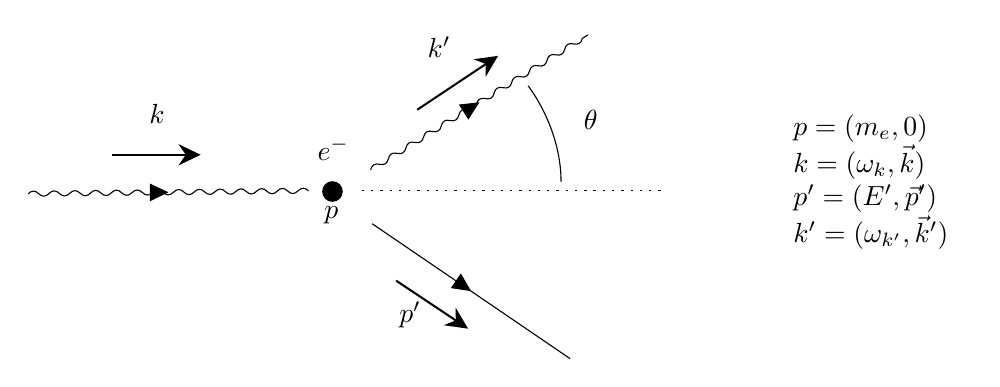
\begin{tikzpicture}[x=0.75pt,y=0.75pt,yscale=-1,xscale=1]
%uncomment if require: \path (0,300); %set diagram left start at 0, and has height of 300

%Straight Lines [id:da47004371895046315] 
\draw    (94,144.56) .. controls (95.65,142.87) and (97.31,142.85) .. (99,144.5) .. controls (100.68,146.15) and (102.35,146.13) .. (104,144.45) .. controls (105.65,142.77) and (107.32,142.75) .. (109,144.4) .. controls (110.69,146.05) and (112.35,146.03) .. (114,144.34) .. controls (115.65,142.66) and (117.32,142.64) .. (119,144.29) .. controls (120.69,145.94) and (122.35,145.92) .. (124,144.23) .. controls (125.65,142.55) and (127.32,142.53) .. (129,144.18) .. controls (130.68,145.83) and (132.35,145.81) .. (134,144.13) .. controls (135.65,142.44) and (137.31,142.42) .. (139,144.07) .. controls (140.68,145.72) and (142.35,145.7) .. (144,144.02) .. controls (145.65,142.34) and (147.32,142.32) .. (149,143.97) .. controls (150.69,145.62) and (152.35,145.6) .. (154,143.91) .. controls (155.65,142.23) and (157.32,142.21) .. (159,143.86) .. controls (160.68,145.51) and (162.35,145.49) .. (164,143.81) .. controls (165.65,142.12) and (167.31,142.1) .. (169,143.75) .. controls (170.68,145.4) and (172.35,145.38) .. (174,143.7) .. controls (175.65,142.02) and (177.32,142) .. (179,143.65) .. controls (180.69,145.3) and (182.35,145.28) .. (183.99,143.59) .. controls (185.64,141.91) and (187.31,141.89) .. (188.99,143.54) .. controls (190.67,145.19) and (192.34,145.17) .. (193.99,143.49) .. controls (195.64,141.8) and (197.3,141.78) .. (198.99,143.43) .. controls (200.67,145.08) and (202.34,145.06) .. (203.99,143.38) .. controls (205.64,141.7) and (207.31,141.68) .. (208.99,143.33) .. controls (210.68,144.98) and (212.34,144.96) .. (213.99,143.27) .. controls (215.64,141.59) and (217.31,141.57) .. (218.99,143.22) .. controls (220.67,144.87) and (222.34,144.85) .. (223.99,143.17) .. controls (225.64,141.48) and (227.3,141.46) .. (228.99,143.11) -- (229.06,143.11) -- (229.06,143.11) ;
\draw [shift={(161.53,143.83)}, rotate = 539.39] [fill={rgb, 255:red, 0; green, 0; blue, 0 }  ][line width=0.08]  [draw opacity=0] (8.93,-4.29) -- (0,0) -- (8.93,4.29) -- cycle    ;
%Flowchart: Connector [id:dp08357812112166041] 
\draw  [fill={rgb, 255:red, 0; green, 0; blue, 0 }  ,fill opacity=1 ] (235.89,143.47) .. controls (235.89,146.06) and (237.99,148.17) .. (240.58,148.17) .. controls (243.18,148.17) and (245.28,146.06) .. (245.28,143.47) .. controls (245.28,140.88) and (243.18,138.78) .. (240.58,138.78) .. controls (237.99,138.78) and (235.89,140.88) .. (235.89,143.47) -- cycle ;
%Straight Lines [id:da8179679192746647] 
\draw    (259,133) .. controls (259.54,130.71) and (260.96,129.83) .. (263.25,130.36) .. controls (265.54,130.9) and (266.96,130.02) .. (267.5,127.73) .. controls (268.03,125.44) and (269.45,124.56) .. (271.74,125.09) .. controls (274.03,125.62) and (275.45,124.74) .. (275.99,122.45) .. controls (276.53,120.16) and (277.95,119.28) .. (280.24,119.82) .. controls (282.53,120.35) and (283.95,119.47) .. (284.49,117.18) .. controls (285.03,114.89) and (286.45,114.01) .. (288.74,114.54) .. controls (291.03,115.08) and (292.45,114.2) .. (292.99,111.91) .. controls (293.52,109.62) and (294.94,108.74) .. (297.23,109.27) .. controls (299.52,109.8) and (300.94,108.92) .. (301.48,106.63) .. controls (302.02,104.34) and (303.44,103.46) .. (305.73,104) .. controls (308.02,104.53) and (309.44,103.65) .. (309.98,101.36) .. controls (310.52,99.07) and (311.94,98.19) .. (314.23,98.72) .. controls (316.52,99.25) and (317.94,98.37) .. (318.47,96.08) .. controls (319.01,93.79) and (320.43,92.91) .. (322.72,93.45) .. controls (325.01,93.98) and (326.43,93.1) .. (326.97,90.81) .. controls (327.51,88.52) and (328.93,87.64) .. (331.22,88.17) .. controls (333.51,88.71) and (334.93,87.83) .. (335.47,85.54) .. controls (336.01,83.25) and (337.43,82.37) .. (339.72,82.9) .. controls (342.01,83.43) and (343.43,82.55) .. (343.96,80.26) .. controls (344.5,77.97) and (345.92,77.09) .. (348.21,77.63) .. controls (350.5,78.16) and (351.92,77.28) .. (352.46,74.99) .. controls (353,72.7) and (354.42,71.82) .. (356.71,72.35) .. controls (359,72.89) and (360.42,72.01) .. (360.96,69.72) -- (363.72,68) -- (363.72,68) ;
\draw [shift={(311.36,100.5)}, rotate = 508.17] [fill={rgb, 255:red, 0; green, 0; blue, 0 }  ][line width=0.08]  [draw opacity=0] (8.93,-4.29) -- (0,0) -- (8.93,4.29) -- cycle    ;
%Straight Lines [id:da15056850292634993] 
\draw  [dash pattern={on 0.84pt off 2.51pt}]  (254.67,143.11) -- (399.83,143.11) ;
%Curve Lines [id:da5581541176414646] 
\draw    (334.83,92.56) .. controls (343.5,104.11) and (350.72,121.44) .. (350.72,138.78) ;
%Straight Lines [id:da0395906445138241] 
\draw    (259.72,159) -- (355.06,224) ;
\draw [shift={(307.39,191.5)}, rotate = 214.29] [fill={rgb, 255:red, 0; green, 0; blue, 0 }  ][line width=0.08]  [draw opacity=0] (8.93,-4.29) -- (0,0) -- (8.93,4.29) -- cycle    ;
%Straight Lines [id:da452390952963887] 
\draw [line width=0.75]    (134.44,125.78) -- (174.06,125.78) ;
\draw [shift={(177.06,125.78)}, rotate = 180] [fill={rgb, 255:red, 0; green, 0; blue, 0 }  ][line width=0.08]  [draw opacity=0] (10.72,-5.15) -- (0,0) -- (10.72,5.15) -- (7.12,0) -- cycle    ;
%Straight Lines [id:da857484560177197] 
\draw [line width=0.75]    (281.39,104.11) -- (317.89,79.78) ;
\draw [shift={(320.39,78.11)}, rotate = 506.31] [fill={rgb, 255:red, 0; green, 0; blue, 0 }  ][line width=0.08]  [draw opacity=0] (10.72,-5.15) -- (0,0) -- (10.72,5.15) -- (7.12,0) -- cycle    ;
%Straight Lines [id:da6224517902495592] 
\draw [line width=0.75]    (271.28,186.44) -- (303.45,207.89) ;
\draw [shift={(305.94,209.56)}, rotate = 213.69] [fill={rgb, 255:red, 0; green, 0; blue, 0 }  ][line width=0.08]  [draw opacity=0] (10.72,-5.15) -- (0,0) -- (10.72,5.15) -- (7.12,0) -- cycle    ;

% Text Node
\draw (365,109) node    {$\theta $};
% Text Node
\draw (156,106) node    {$k$};
% Text Node
\draw (292,74) node    {$k'$};
% Text Node
\draw (278,203) node    {$p'$};
% Text Node
\draw (241,123) node    {$e^{-}$};
% Text Node
\draw (240,155) node    {$p$};
%Text Node
\draw (500,139) node    {$ \begin{array}{l}
p=( m_{e} ,0)\\
k=( \omega _{k} ,\vec{k})\\
p'=( E',\vec{p} ')\\
k'=( \omega _{k'} ,\vec{k} ')
\end{array}$};


\end{tikzpicture}
\end{figure}

We will express the cross section in terms of $\omega$ and $\theta$. We can find $\omega'$, the energy of the final photon, using the following trick:
\begin{align*}
m^2&=(p')^2=(p+k-k')^2=p^2+2p\cdot(k-k')-2k\cdot k'\\
&=m^2+2m(\omega_k-\omega_{k'})-2\omega_k\omega_{k'}(1-\cos\theta)
\end{align*}
hence, we obtain Compton's formula for the shift in the photon wavelength:
\[\Delta\lambda=\left(\frac1{\omega_{k'}}-\frac1{\omega_{k}}\right)=\frac{1-\cos\theta}{m}\]
For our purposes, however, is more useful to solve for $\omega_{k'}$:
\begin{equation}\label{eqn:QED-compton-energies-lab}
\omega_{k'}=\frac{\omega_k}{1+\frac{\omega_{k}}m(1-\cos\theta)}
\end{equation}

The unpolarized amplitude in the Lab frame is
\begin{align*}
|\bar{\mathcal M}|_{\textup{LAB}}^2&=2q^4\left[\left(\frac{\omega_{k'}}{\omega_k}+\frac{\omega_k}{\omega_{k'}}\right)+2m\left(\frac1{\omega_k}-\frac1{\omega_{k'}}\right)+m^2\left(\frac1{\omega_k}-\frac1{\omega_{k'}}\right)^2\right]\\
&=2q^4\left[\left(\frac{\omega_{k'}}{\omega_k}+\frac{\omega_k}{\omega_{k'}}\right)-\sin^2\theta\right]
\end{align*}

The covariant flux factor reads
\[I_{\textup{LAB}}=[(p\cdot k)^2-m_e^2m_\gamma^2]^{1/2}=|p\cdot k|=m_e\omega_k\]
The 2-body phase space
\begin{align*}
\int\de\Phi_{(2)}&=\int \frac{\de^3k'}{(2\pi)^32\omega_{k'}}\frac{\de^3p'}{(2\pi)^32E'}(2\pi)^4\delta^4(k'+p'-k-p)
=\int\frac{\omega^2_{k'}\de\omega_{k'}\de\Omega}{(2\pi)^2}\frac{1}{4\omega_{k'}E'}\delta(\omega_{k'}+E'-\omega_k-m)\\
&=\int\frac{\omega^2_{k'}\de\omega_{k'}\de\Omega}{(2\pi)^2}\frac{1}{4\omega_{k'}E'}\frac{\delta(\omega_{k'}-|\vec k'|)}{\left|\frac{\partial(\omega_{k'}+E'-\omega_k-m)}{\partial|k'|}\right|}_{\omega_{k'}=|\vec k'|}
=\int\de\Omega\frac{|\vec k'|^2}{16\pi^2\omega_{k'}E'}\left|\frac{\partial(\omega_{k'}+E')}{\partial|k'|}\right|^{-1}_{\omega_{k'}=|\vec k'|}
\end{align*}
where 
\[E'=\left(m^2+(\vec k-\vec k')^2\right)^{1/2}
=\left[m^2+\omega_k^2+\omega_{k'}^2-2\omega_{k'}\omega_k\cos\theta\right]^{1/2}\]
\[\frac{\partial E'}{\partial|k'|}=\frac{\omega_{k'}-\omega_k\cos\theta}{E'}\]
and
\todo{Controlla l'ultimo passaggio}

\[\left|\frac{\partial(\omega_{k'}+E')}{\partial|k'|}\right|_{\omega_{k'}=|\vec k'|}
=\left|1+\frac{\omega_{k'}-\omega_k\cos\theta}{E'}\right|
=\frac{m\omega_k}{E'\omega_{k'}}
\]
So the unpolarized cross section is 
\begin{align*}
\left(\frac{\de\bar\sigma}{\de\Omega}\right)_{\textup{LAB}}&=
\frac{\overline{|\mathcal M|}_{\textup{LAB}}^2}{4I_{\textup{LAB}}}\frac{\de\Phi_{(2)}}{\de\Omega}
=\frac1{64\pi^2}\frac{|\vec k'|^2}{I_{\textup{LAB}}\omega_{k'}E'}\left|\frac{\partial(\omega_{k'}+E')}{\partial|k'|}\right|^{-1}\overline{|\mathcal M|}_{\textup{LAB}}^2\\
&=\frac{q^4}{32\pi^2}\frac1{m^2}\left(\frac{\omega_{k'}}{\omega_k}\right)^2\left(\frac{\omega_{k'}}{\omega_k}+\frac{\omega_k}{\omega_{k'}}-\sin^2\theta\right)\\
&=\frac{\alpha^2}{2}\frac1{m^2}\left(\frac{\omega_{k'}}{\omega_k}\right)^2\left(\frac{\omega_{k'}}{\omega_k}+\frac{\omega_k}{\omega_{k'}}-\sin^2\theta\right)
\end{align*}
where $\omega_{k'}/\omega_{k}$ is given by \eqref{eqn:QED-compton-energies-lab} and in the last step we used $\alpha=e^2/(4\pi)$. Writing $\de\Omega=(2\pi)\de\cos\theta$ we obtain
\begin{align}\label{eqn:Klein-Nishina}
\left(\frac{\de\bar\sigma}{\de\cos\theta}\right)_{\textup{LAB}}&=
\frac{\pi\alpha^2}{m^2}\left(\frac{\omega_{k'}}{\omega_k}\right)^2\left(\frac{\omega_{k'}}{\omega_k}+\frac{\omega_k}{\omega_{k'}}-\sin^2\theta\right)
\end{align}

This is the (spin-averaged) \emph{Klein-Nishina formula}.
In the low energy limit $\omega_k\ll m$, from \eqref{eqn:QED-compton-energies-lab} we have $\omega_{k'}\approx\omega_{k}$, i.e. the kinetic energy of the recoil electron is negligible, and Eq.\eqref{eqn:Klein-Nishina} reduces to the familiar Thomson cross-section for scattering of classical electromagnetic radiation by a free electron:

\begin{align*}
\left(\frac{\de\bar\sigma}{\de\cos\theta}\right)_{\textup{LAB}}&\overset{\omega_k\ll m}{=}
\frac{\pi\alpha^2}{m^2}\left(1+\cos^2\theta\right)
\quad\rightarrow\quad
(\bar\sigma)_{\textup{LAB}}=\frac{8\pi\alpha^2}{3m^2}\equiv\frac83\pi r_e^2
\end{align*}

We have calculated the full relativistic corrections for the Thomson formula.

\subsection{C.o.M. frame - High energy photon}
\textsf{See Peskin sec. 5.5, and Schwartz sec. 13.5.4}
To analyze the high-energy behaviour of the Compton scattering cross section, it is easiest to work in the center-of-mass frame.

\begin{figure}[H]
\centering


\tikzset{every picture/.style={line width=0.75pt}} %set default line width to 0.75pt        

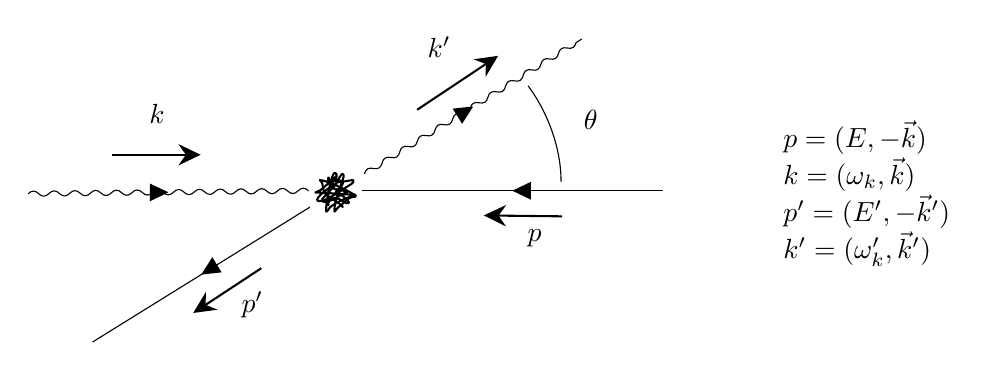
\begin{tikzpicture}[x=0.75pt,y=0.75pt,yscale=-1,xscale=1]
%uncomment if require: \path (0,300); %set diagram left start at 0, and has height of 300

%Straight Lines [id:da2201162405089543] 
\draw    (94,144.56) .. controls (95.65,142.87) and (97.31,142.85) .. (99,144.5) .. controls (100.68,146.15) and (102.35,146.13) .. (104,144.45) .. controls (105.65,142.77) and (107.32,142.75) .. (109,144.4) .. controls (110.69,146.05) and (112.35,146.03) .. (114,144.34) .. controls (115.65,142.66) and (117.32,142.64) .. (119,144.29) .. controls (120.69,145.94) and (122.35,145.92) .. (124,144.23) .. controls (125.65,142.55) and (127.32,142.53) .. (129,144.18) .. controls (130.68,145.83) and (132.35,145.81) .. (134,144.13) .. controls (135.65,142.44) and (137.31,142.42) .. (139,144.07) .. controls (140.68,145.72) and (142.35,145.7) .. (144,144.02) .. controls (145.65,142.34) and (147.32,142.32) .. (149,143.97) .. controls (150.69,145.62) and (152.35,145.6) .. (154,143.91) .. controls (155.65,142.23) and (157.32,142.21) .. (159,143.86) .. controls (160.68,145.51) and (162.35,145.49) .. (164,143.81) .. controls (165.65,142.12) and (167.31,142.1) .. (169,143.75) .. controls (170.68,145.4) and (172.35,145.38) .. (174,143.7) .. controls (175.65,142.02) and (177.32,142) .. (179,143.65) .. controls (180.69,145.3) and (182.35,145.28) .. (183.99,143.59) .. controls (185.64,141.91) and (187.31,141.89) .. (188.99,143.54) .. controls (190.67,145.19) and (192.34,145.17) .. (193.99,143.49) .. controls (195.64,141.8) and (197.3,141.78) .. (198.99,143.43) .. controls (200.67,145.08) and (202.34,145.06) .. (203.99,143.38) .. controls (205.64,141.7) and (207.31,141.68) .. (208.99,143.33) .. controls (210.68,144.98) and (212.34,144.96) .. (213.99,143.27) .. controls (215.64,141.59) and (217.31,141.57) .. (218.99,143.22) .. controls (220.67,144.87) and (222.34,144.85) .. (223.99,143.17) .. controls (225.64,141.48) and (227.3,141.46) .. (228.99,143.11) -- (229.06,143.11) -- (229.06,143.11) ;
\draw [shift={(161.53,143.83)}, rotate = 539.39] [fill={rgb, 255:red, 0; green, 0; blue, 0 }  ][line width=0.08]  [draw opacity=0] (8.93,-4.29) -- (0,0) -- (8.93,4.29) -- cycle    ;
%Straight Lines [id:da8440776864610582] 
\draw    (256,135) .. controls (256.54,132.71) and (257.96,131.83) .. (260.25,132.36) .. controls (262.54,132.9) and (263.96,132.02) .. (264.5,129.73) .. controls (265.03,127.44) and (266.45,126.56) .. (268.74,127.09) .. controls (271.03,127.62) and (272.45,126.74) .. (272.99,124.45) .. controls (273.53,122.16) and (274.95,121.28) .. (277.24,121.82) .. controls (279.53,122.35) and (280.95,121.47) .. (281.49,119.18) .. controls (282.03,116.89) and (283.45,116.01) .. (285.74,116.54) .. controls (288.03,117.08) and (289.45,116.2) .. (289.99,113.91) .. controls (290.52,111.62) and (291.94,110.74) .. (294.23,111.27) .. controls (296.52,111.8) and (297.94,110.92) .. (298.48,108.63) .. controls (299.02,106.34) and (300.44,105.46) .. (302.73,106) .. controls (305.02,106.53) and (306.44,105.65) .. (306.98,103.36) .. controls (307.52,101.07) and (308.94,100.19) .. (311.23,100.72) .. controls (313.52,101.25) and (314.94,100.37) .. (315.47,98.08) .. controls (316.01,95.79) and (317.43,94.91) .. (319.72,95.45) .. controls (322.01,95.98) and (323.43,95.1) .. (323.97,92.81) .. controls (324.51,90.52) and (325.93,89.64) .. (328.22,90.17) .. controls (330.51,90.71) and (331.93,89.83) .. (332.47,87.54) .. controls (333.01,85.25) and (334.43,84.37) .. (336.72,84.9) .. controls (339.01,85.43) and (340.43,84.55) .. (340.96,82.26) .. controls (341.5,79.97) and (342.92,79.09) .. (345.21,79.63) .. controls (347.5,80.16) and (348.92,79.28) .. (349.46,76.99) .. controls (350,74.7) and (351.42,73.82) .. (353.71,74.35) .. controls (356,74.89) and (357.42,74.01) .. (357.96,71.72) -- (360.72,70) -- (360.72,70) ;
\draw [shift={(308.36,102.5)}, rotate = 508.17] [fill={rgb, 255:red, 0; green, 0; blue, 0 }  ][line width=0.08]  [draw opacity=0] (8.93,-4.29) -- (0,0) -- (8.93,4.29) -- cycle    ;
%Straight Lines [id:da09307133911969756] 
\draw    (254.67,143.11) -- (399.83,143.11) ;
\draw [shift={(327.25,143.11)}, rotate = 0] [fill={rgb, 255:red, 0; green, 0; blue, 0 }  ][line width=0.08]  [draw opacity=0] (8.93,-4.29) -- (0,0) -- (8.93,4.29) -- cycle    ;
%Curve Lines [id:da33812291607616296] 
\draw    (334.83,92.56) .. controls (343.5,104.11) and (350.72,121.44) .. (350.72,138.78) ;
%Straight Lines [id:da5774490131113152] 
\draw [line width=0.75]    (134.44,125.78) -- (174.06,125.78) ;
\draw [shift={(177.06,125.78)}, rotate = 180] [fill={rgb, 255:red, 0; green, 0; blue, 0 }  ][line width=0.08]  [draw opacity=0] (10.72,-5.15) -- (0,0) -- (10.72,5.15) -- (7.12,0) -- cycle    ;
%Straight Lines [id:da24269378260147034] 
\draw [line width=0.75]    (281.39,104.11) -- (317.89,79.78) ;
\draw [shift={(320.39,78.11)}, rotate = 506.31] [fill={rgb, 255:red, 0; green, 0; blue, 0 }  ][line width=0.08]  [draw opacity=0] (10.72,-5.15) -- (0,0) -- (10.72,5.15) -- (7.12,0) -- cycle    ;
%Straight Lines [id:da3757335905736008] 
\draw [line width=0.75]    (206.28,180.44) -- (176.01,200.35) ;
\draw [shift={(173.5,202)}, rotate = 326.66999999999996] [fill={rgb, 255:red, 0; green, 0; blue, 0 }  ][line width=0.08]  [draw opacity=0] (10.72,-5.15) -- (0,0) -- (10.72,5.15) -- (7.12,0) -- cycle    ;
%Straight Lines [id:da04091628549293125] 
\draw    (125,216) -- (229.72,151) ;
\draw [shift={(177.36,183.5)}, rotate = 328.17] [fill={rgb, 255:red, 0; green, 0; blue, 0 }  ][line width=0.08]  [draw opacity=0] (8.93,-4.29) -- (0,0) -- (8.93,4.29) -- cycle    ;
%Straight Lines [id:da587248071756918] 
\draw [line width=0.75]    (351.28,155.44) -- (316.5,155.04) ;
\draw [shift={(313.5,155)}, rotate = 360.66999999999996] [fill={rgb, 255:red, 0; green, 0; blue, 0 }  ][line width=0.08]  [draw opacity=0] (10.72,-5.15) -- (0,0) -- (10.72,5.15) -- (7.12,0) -- cycle    ;
%Shape: Free Drawing [id:dp672077562881797] 
\draw  [color={rgb, 255:red, 0; green, 0; blue, 0 }  ][line width=0.75] [line join = round][line cap = round] (238.5,139) .. controls (238.5,134.42) and (238.79,137.16) .. (239.5,140) .. controls (239.61,140.46) and (240.17,139.33) .. (240.5,139) .. controls (241.52,137.98) and (244.74,137.49) .. (245.5,139) .. controls (246.37,140.74) and (240.56,144) .. (242.5,144) .. controls (244.25,144) and (249.12,148.69) .. (248.5,149) .. controls (246.85,149.82) and (245.13,147.33) .. (243.5,147) .. controls (242.19,146.74) and (240.69,146.4) .. (239.5,147) .. controls (238.56,147.47) and (238.5,151.05) .. (238.5,150) .. controls (238.5,145.09) and (238.54,139.96) .. (241.5,137) .. controls (241.83,136.67) and (242.5,136) .. (242.5,136) .. controls (242.5,136) and (235.39,142.55) .. (234.5,143) .. controls (233.83,143.33) and (231.75,144) .. (232.5,144) .. controls (238.77,144) and (245.98,145) .. (251.5,145) .. controls (253.3,145) and (248.11,146.2) .. (246.5,147) .. controls (244.9,147.8) and (240.81,149.69) .. (239.5,151) .. controls (238.83,151.67) and (237.73,153.91) .. (237.5,153) .. controls (237.11,151.43) and (240.32,130.65) .. (242.5,135) .. controls (243.1,136.19) and (241.39,138.26) .. (242.5,139) .. controls (243.03,139.35) and (250.31,137.81) .. (250.5,138) .. controls (251.19,138.69) and (249.76,139.87) .. (249.5,140) .. controls (247.14,141.18) and (236.38,149.44) .. (233.5,148) .. controls (231.39,146.95) and (240.55,140) .. (242.5,140) ;
%Shape: Free Drawing [id:dp3629185907562005] 
\draw  [color={rgb, 255:red, 0; green, 0; blue, 0 }  ][line width=0.75] [line join = round][line cap = round] (245.5,151) .. controls (245.5,149.77) and (238.43,145.93) .. (237.5,145) .. controls (235.85,143.35) and (236.16,140.97) .. (235.5,139) .. controls (235.35,138.55) and (234.03,138) .. (234.5,138) .. controls (237.62,138) and (245.48,141.99) .. (247.5,143) .. controls (248.99,143.75) and (253.17,146) .. (251.5,146) .. controls (247.23,146) and (245.77,149.87) .. (243.5,151) .. controls (242.66,151.42) and (241.5,153.94) .. (241.5,153) .. controls (241.5,147.47) and (243.79,143.12) .. (245.5,138) .. controls (245.82,137.05) and (246.39,135.45) .. (245.5,135) .. controls (244.77,134.63) and (241.54,140.96) .. (241.5,141) .. controls (240.88,141.62) and (234.76,147.26) .. (235.5,148) .. controls (237.89,150.39) and (245.38,144) .. (247.5,144) .. controls (248.25,144) and (246.21,143.24) .. (245.5,143) .. controls (243.55,142.35) and (241.34,142.84) .. (239.5,141) ;

% Text Node
\draw (365,109) node    {$\theta $};
% Text Node
\draw (156,106) node    {$k$};
% Text Node
\draw (292,74) node    {$k'$};
% Text Node
\draw (202,198) node    {$p'$};
% Text Node
\draw (338,166) node    {$p$};
% Text Node
\draw (498,145) node    {$ \begin{array}{l}
p=( E,-\vec{k})\\
k=( \omega _{k} ,\vec{k})\\
p'=( E',-\vec{k} ')\\
k'=( \omega _{k} ',\vec{k} ')
\end{array}$};


\end{tikzpicture}
\end{figure}

The kinematics of the reaction in the high energy limit ($m\approx0$) looks like
\begin{align*}
E&=\sqrt{\vec k^2+m^2}\overset{m=0}{\approx}|\vec k|=\omega_k\\
E'&=\sqrt{\vec k'^2+m^2}\overset{m=0}{\approx}|\vec k'|=\omega_{k'}
\end{align*}
\begin{align*}
p\cdot k\,&=E\omega_k+|\vec k|^2=\omega_k(E+\omega_k)\overset{m=0}{\approx}2\omega_k^2\\
p\cdot p'&=E\,E'-\vec k\vec k'=E\,E'-|\vec k||\vec k'|\cos\theta=E\,E'-\omega_k\omega_{k'}\cos\theta\overset{m=0}{\approx}\omega_k\omega_{k'}(1-\cos\theta)\\
p\cdot k'&=E\,\omega_{k'}+\vec k\vec k'=E\,\omega_{k'}+|\vec k||\vec k'|\cos\theta=\omega_{k'}(E+\omega_k\cos\theta)\overset{m=0}{\approx}\omega_k\omega_{k'}(1+\cos\theta)
\end{align*}
We also have
\begin{align*}
s&=(p+k)^2=m^2+2p\cdot k=m^2+2\omega_k(E+\omega_k)\overset{m=0}{\approx}4\omega_k^2 \quad\rightarrow\quad \omega_k\overset{m=0}{\approx}\frac{\sqrt s}{2}\\
s&=(p'+k')^2=m^2+2p'\cdot k'=m^2+2\omega_{k'}(E'+\omega_k')\overset{m=0}{\approx}4\omega_{k'}^2 \quad\rightarrow\quad \omega_{k'}\overset{m=0}{\approx}\frac{\sqrt s}{2}
\end{align*}

Plugging these values into Eq.\eqref{eqn:Compton-unpolarized-squared}

\begin{align*}
\overline{|\mathcal M|}^2
&=2q^4\left[\frac{p\cdot k'}{p\cdot k}+\frac{p\cdot k}{p\cdot k'}+2m^2\left(\frac1{p\cdot k}-\frac1{p\cdot k'}\right)+m^4\left(\frac1{p\cdot k}-\frac1{p\cdot k'}\right)^2\right]
\end{align*}

for c.o.m. frame with $E\gg m$ we have 
\begin{align*}
\overline{|\mathcal M|}_{\textup{CM}}^2
&\approx2q^4\left(\frac{p\cdot k'}{p\cdot k}+\frac{p\cdot k}{p\cdot k'}\right)\approx2q^4\left(\frac{1+\cos\theta}{2}+\frac{2}{1+\cos\theta}\right)
\end{align*}

we notice that the term $p\cdot k/p\cdot k'$ becomes divergent when the electron is emitted in the backward direction ($\theta\approx\pi$), while other terms are all of $\mathcal O(1)$ or smaller.

Notice that two initial diagrams $\mathcal M_A$, $s$-channel, and $\mathcal M_B$, $u$-channel, give contributions to the total amplitude proportional to\footnote{You can easily verify this statement looking at the calculation on the beginning of this section.} 
\[\mathcal M_A\quad\rightarrow\quad\frac1{2p\cdot k}=\frac1{s-m^2}\qquad\quad
\mathcal M_B\quad\rightarrow\quad\frac1{2p\cdot k'}=\frac1{u-m^2}\]
Here is clear the relation between the momentum of the channel and the contribution to the total Feynman amplitude. The divergent contribution is due to the square of the $u$-channel diagram, we can see that for $\theta=\pi$ we have $u=(p-k')^2=m^2-2p\cdot k'\approx m^2-2\omega_k^2(1+\cos\theta)\approx m^2$ i.e. the divergent contribution is related to the situation where the initial electron emits a photon with all its kinetic energy and then absorbs all the energy of the initial photon. The amplitude is large at $\theta\approx\pi$ because the denominator of the propagator is then small ($\sim m^2$) compared to $s$. This kind of divergence is called \emph{Infra-Red divergence}.\\
\todo{This is a Infra-Red divergence, related to Sudakov logs. Add some comment. See Mandl 8.9}
We can correct the divergent term (unphysical) considering higher terms in the Taylor expantion of $E$ in $m$:
\begin{align*}
E&=\sqrt{\vec k^2+m^2}=|\vec k|+\frac{m^2}{2|\vec k|}+o(m^3)\overset{m\approx0}{\approx}\omega_k+\frac{m^2}{2\omega_k}
\end{align*}
\[p\cdot k'=\omega_{k'}(E+\omega_k\cos\theta)\overset{m=0}{\approx}\omega_{k'}\left(\omega_k+\frac{m^2}{2\omega_k}+\omega_k\cos\theta\right)
=\omega_{k}^2\left(1+\cos\theta+\frac{m^2}{2\omega_k^2}\right)\]
\begin{align*}
\overline{|\mathcal M|}_{\textup{CM}}^2
&\approx2q^4\left(\frac{p\cdot k'}{p\cdot k}+\frac{p\cdot k}{p\cdot k'}\right)
\approx2q^4\left(\frac{1+\cos\theta}{2}+\frac{2}{1+\cos\theta+\frac{m^2}{2\omega_k^2}}\right)
\end{align*}
Now we can compute the cross section in the CM frame (we can use the formula for elastic scattering):
\begin{align*}
\left(\frac{\de\bar\sigma}{\de\Omega}\right)_{\textup{CM}}
=\frac1{64\pi^2}\frac{\overline{|\mathcal M|}^2_{\textup{CM}}}s
&\approx\frac{q^4}{32\pi^2s}\left(\frac{1+\cos\theta}{2}+\frac{2}{1+\cos\theta+\frac{m^2}{2\omega_k^2}}\right)\\
&\approx\frac{\alpha^2}{2s}\left(\frac{1+\cos\theta}{2}+\frac{2}{1+\cos\theta+\frac{m^2}{2\omega_k^2}}\right)
\end{align*}
or
\[{\left(\frac{\de\bar\sigma}{\de(\cos\theta)}\right)}_{\textup{CM}}
\approx\frac{\pi\alpha^2}{s}\left(\frac{1+\cos\theta}{2}+\frac{2}{1+\cos\theta+\frac{m^2}{2\omega_k^2}}\right)\]
Recall that the electron mass $m$ can be neglected completely in this formula if it were not necessary to cutoff the singularity for $\theta=0$.\\
The total Compton scattering cross section reads:
\begin{align*}
\bar\sigma_{\textup{total}}=\int_{-1}^1\de(\cos\theta){\left(\frac{\de\bar\sigma}{\de(\cos\theta)}\right)}_{\textup{CM}}
&\approx 
\frac{\pi\alpha^2}{s}\int_{-1}^1\de(\cos\theta)\left(\frac{1+\cos\theta}{2}+\frac{2}{1+\cos\theta+\frac{m^2}{2\omega_k^2}}\right)\\
&=\frac{\pi\alpha^2}{s}+\frac{2\pi\alpha^2}{s}\log\left(\frac s{m^2}\right)
\end{align*}
The main dependence $\alpha^2/s$ follows from dimensional analysis. But the singularity associated to backward scattering of photons leads to an enhancement by an extra logarithm of the energy, called \emph{Sudakov logarithm}.

\todo{Inserire diagrammi di Feynman pag 168 Peskin (ruotati appropriatamente)}
\begin{exercise}[Pair Annihilation into Photons]
Find the total cross section of the annihilation process $e^+e^-\rightarrow2\gamma$
\end{exercise}


\section{Scattering by an external E.M. field and the Rutherford formula}
\textsf{See Mandl sec. 8.7 and Schwartz sec. 13.4}

Now let us go back to the problem of scattering of an electron by a Coulomb potential. Recall the classical Rutherford scattering formula, 
\[\frac{\de\sigma}{\de\Omega}=\frac{m_e^2e^4}{4|\vec p_i|^4\sin^4\frac\theta2}\]
where $|\vec p_i|=|\vec p_f|$ is the magnitude of the incoming electron momentum, which. is the same as the magnitude of the outgoing electron momentum for elastic scattering. Rutherford calculated this using classical mechanics to describe how an electron would get deflected in a central potential, as from atomic nucleus.

In order to give a description of this process using QED, we modify the QED lagrangian, so that we introduce also protons in our theory. We consider a low energy process, where the proton can be consider as a fundamental particle, described as a spin $1/2$ fermion. Then we can do the same trick we used for QED flavours. The modified Lagrangian reads:
\[\mathcal L=\bar\psi_e(i\slashed\partial-m_e)\psi_e+\bar\psi_p(i\slashed\partial-M_p)\psi_p+\underbrace{q_e\bar\psi_e\slashed A\psi_e+q_p\bar\psi_p\slashed A\psi_p}_{\mathcal L_{\textup{int}}}\]

{\small Notice that $\mathcal L_{\textup{int}}$ in order to obtain a description of Rutherford scattering we need to consider at least 2-nd order processes, i.e. 2 vertex.}
The two-vertex S matrix element becomes
\begin{align*}
S_{(2)}&=\frac{(-i)^2}{2!}\int\de^4 x\,\de^4y\,\textup{T}\left\{\textup{N}\left[q_e\bar\psi_e\slashed A\psi_e+q_p\bar\psi_p\slashed A\psi_p\right]_x\textup{N}\left[q_e\bar\psi_e\slashed A\psi_e+q_p\bar\psi_p\slashed A\psi_p\right]_y\right\}\\
&=\frac12(-iq_e)(-iq_p)\int\de^4 x\,\de^4y\,\textup{T}\left\{\textup{N}\left[\bar\psi_e\slashed A\psi_e\right]_x\textup{N}\left[\bar\psi_p\slashed A\psi_p\right]_y+\textup{N}\left[\bar\psi_e\slashed A\psi_e\right]_y\textup{N}\left[\bar\psi_p\slashed A\psi_p\right]_x\right\}\\
&=(-iq_e)(-iq_p)\int\de^4 x\,\de^4y\,\textup{T}\left\{\textup{N}\left[\bar\psi_e\slashed A\psi_e\right]_x\textup{N}\left[\bar\psi_p\slashed A\psi_p\right]_y\right\}
\end{align*}
%
where in the first step we omitted products in the integral that does not describe interaction between electron and proton, and in the second step we change integral variables in the second term of the time product.

The $e^-p\rightarrow e^-p$  process is similar to the process $e^-f^-\rightarrow e^-f^-$. Both processes are described by a $t$-channel

\begin{figure}[H]
\centering
\begin{tikzpicture}[baseline=(i)]
  \begin{feynman}[large]
    \vertex (e1) {\(e^-\)};
    \vertex [label={[label distance=0cm]182:$\mu$}] at ([shift={(315:2.5)}]e1)  (mu);
    \vertex [label={[label distance=0.1cm]270:$\nu$}] at ([shift={(270:2)}]mu) (nu);
    \vertex [below right=of nu] (p2) {\(p\)};
    \vertex [below left=of nu] (p1){\(p\)};
    \vertex [above right=of mu] (e2){\(e^-\)};
    \vertex at ([shift={(270:1)}]mu)(i);
    
    \diagram*{
      (e1) -- [fermion, momentum={[arrow shorten=0.25]\(p_e\)}] (mu) -- [fermion, momentum={[arrow shorten=0.2]\(p_e'\)}](e2),
      (mu) -- [boson, momentum={[arrow shorten=0.3]\(k=(p-p')=(q'-q)=\sqrt t\)}] (nu),
      (p1) -- [fermion, ultra thick, red, momentum={[arrow shorten=0.25, black]\(p_p\)}] (nu) -- [fermion, ultra thick, red, momentum={[arrow shorten=0.2, black]\(p_p'\)}](p2),
      };
  \end{feynman}
\end{tikzpicture}
\end{figure}





















\end{document}